\chapter{Introdução}

\section{Motivação}
\label{sec:motivacao}

As cidades são repletas de agentes, cada um com diferentes interesses. Os cidadãos desejam maximizar a qualidade de vida, o que geralmente significa habitar residências espaçosas, em lugares tranquilos, repletos de natureza, mas que ainda tenham acesso às oportunidades de emprego, lazer, saúde, educação, entre outros. As imobiliárias e construtoras desejam construir prédios, casas e condomínios que maximizem seus lucros, escolhendo as localizações com maior demanda e menores custos. Os proprietários de terras e imóveis buscam comprar ativos baratos com a expectativa de que valorizem no futuro ou extraiam renda de aluguel. 

Porém, a dinâmica das cidades é moldada por inúmeros conflitos de interesses, visto que muitos deles são antagônicos. É impossível, por exemplo, que todo mundo more em contato com a natureza, já que na medida em que cada família constrói sua casa, a natureza do vizinho diminui. Dessa forma, há duas maneiras de coexistir no espaço: através das relações de poder, nas quais, o agente mais poderoso tem seu interesse atendido (ou negociado) em detrimento de outro, ou um planejador central intermedeia este conflito de forma a gerar o resultado mais favorável para todos.

A principal instituição responsável por intermediar os conflitos da esfera urbana de São Paulo, a cidade mais populosa das Américas, é o Plano Diretor Estratégico (PDE). O PDE é uma lei municipal que institui as regras da cidade como o zoneamento e regulações sobre padrões construtivos. O plano diretor de 2014 trouxe mudanças significativas em relação ao seu predecessor, de 2002, sendo reconhecido internacionalmente pela sua abordagem de combate às desigualdades e incentivo ao uso do transporte público.

Enquanto o plano de 2002 descentralizou grande parte das decisões sobre zoneamento nas subprefeituras, o PDE de 2014 seguiu uma abordagem moderna, em linha com a literatura do urbanismo de \textit{Transit Oriented Development} (TOD), em português, ``desenvolvimento orientado ao transporte''. Antigamente, cada subprefeitura teria protagonismo no zoneamento de sua região, enquanto no novo plano, a regulação foi definida a nível municipal e centralizado. O sistema antigo apresentava grande dificuldade em lidar com os conflitos de interesse e grupos locais tinham a capacidade de conter o adensamento em áreas desejáveis\footnote{Movimento conhecido como \textit{Not in My Backyard} (NIMBY), em português, ``não no meu quintal''.}, prejudicando o desenvolvimento sustentável da cidade.

A literatura de TOD, que surgiu no final da década de 80, mas popularizou-se apenas depois dos anos 2000, defende a mobilidade como um dos principais pilares do desenvolvimento das cidades \cite{Ibraeva2020}. A proposta do TOD é aproximar as famílias às oportunidades, através do direcionamento do desenvolvimento urbano no entorno de infraestrutura de transporte coletivo de alta capacidade, causando uma melhora na mobilidade e maior adensamento. Dessa forma, diminui-se a dependência do transporte individual motorizado, que gera externalidades negativas.

As ideias do TOD não apenas influenciam o PDE de 2014, como são uma parte estruturante. Entre os objetivos enunciados do plano diretor, destacam-se os quatro primeiros:

{\small
\begin{quote}
    Art. 7º A Política de Desenvolvimento Urbano 
    e o Plano Diretor Estratégico se orientam pelos 
    seguintes objetivos estratégicos:

    I - conter o processo de expansão horizontal da aglomeração urbana, contribuindo para preservar o cinturão verde metropolitano;

    II - acomodar o crescimento urbano nas áreas subutilizadas dotadas de infraestrutura e no entorno da rede de transporte coletivo de alta e média capacidade

    III - reduzir a necessidade de deslocamento, equilibrando a relação entre os locais de emprego e de moradia;

    IV - expandir as redes de transporte coletivo de alta e média capacidade e os modos não motorizados, racionalizando o uso de automóvel;
\end{quote}
}
Dito isso, a pergunta motivadora desta pesquisa é se 10 anos depois do início da vigência do plano diretor é possível identificar se ele está cumprindo com seus objetivos -- em especial, o objetivo de adensar as áreas na proximidade da infraestrutura de transporte público.

\section{Plano Diretor Estratégico (PDE)}
\label{sec:plano-diretor}

Esta seção é dedicada a compreender quais ferramentas estão à disposição do plano diretor para que alcance seus objetivos \cite{PDE2002, PDE2014, PDE2023}. Todavia, o PDE apresenta diversos instrumentos que agem não apenas em prédios novos, como também atua na requalificação de lotes já construídos. O foco desta pesquisa está nos três principais instrumentos desenhados para a regulamentação de novas construções. Estes são o coeficiente de aproveitamento, a cota parte e o gabarito. Outros instrumentos, apesar de importantes, não têm como objetivo regular a densidade populacional de cada área. 

O PDE dividiu o mapa da cidade em macroáreas, macrozonas e zonas especiais, cada uma com objetivos específicos e respectivas restrições para cada instrumento. Além disso, criou um regime especial para lotes que estejam próximos à infraestrutura de transporte público de alta capacidade, região nomeada de Eixos de Estruturação da Transformação Urbana (EETUs). 

\subsection*{Eixos de Estruturação da Transformação Urbana (EETUs)}

Os eixos são definidos pela proximidade ao transporte público de alta capacidade, e em São Paulo essa ativação ocorre de duas formas. A primeira é por meio de estações de trem, metrô ou monotrilho, que criam uma área de influência com um raio de 400 metros ao redor dos pontos de acesso. A segunda ocorre através de corredores de ônibus municipais e intermunicipais, que geram uma área de influência de 150 metros para cada lado da via ao longo do corredor.

Nas zonas dos eixos, além de existir um regime especial para os três instrumentos que serão apresentados, são implementadas outras medidas para incentivar o uso do transporte coletivo. Por exemplo, para desestimular o uso de carros, foram criadas restrições ao número de vagas de estacionamento, que anteriormente eram incentivadas pelo PDE de 2002. Assim, os eixos se tornam áreas de teste para a eficácia desses instrumentos, já que são aplicados em seu pleno potencial.

\subsection*{Coeficiente de Aproveitamento (CA)}

O Coeficiente de Aproveitamento (CA) é um instrumento utilizado mundialmente\footnote{Em inglês, \textit{Floor Area Ratio} (FAR) ou \textit{Floor Area Ratio}.} em planos diretores para regular a \textbf{densidade construtiva}. O CA determina quantas vezes a área do lote pode ser construída. A legislação paulistana prescreve no direito de propriedade de todos os lotes da cidade um coeficiente de aproveitamento básico igual a 1, ou seja, é permitido construir uma vez a área do terreno. Se um proprietário desejar construir 4 andares em seu lote, com uma CA de 1, pode ocupar apenas 1/4 da área do terreno. Na ótica da legislação, o potencial de construir metros quadrados a mais de uma vez a área do terreno não está incluso no direito de propriedade, e, portanto pertence à sociedade, não ao proprietário do lote.

Em cada macroárea da cidade há restrições diferentes para o CA mínimo e máximo -- o básico se mantém 1 em toda a cidade. Na Macrozona de Estruturação e Qualificação Urbana, o CA mínimo varia entre 0,3 e 0,5 a depender de qual macroárea se encontra, e o máximo é sempre 2. Na Macrozona de Proteção e Recuperação Ambiental, não há CA mínimo e o CA máximo varia entre 0,1 e 1, a depender do nível de proteção que foi designado à região. Nessas áreas de preservação outras regulações também podem atuar\footnote{Aplica-se a legislação estadual pertinente, especialmente as leis específicas das Bacias Billings e Guarapiranga.}.

Quando a região é ativada por transporte público de alta capacidade, há modificadores sobre o CA. Na Macrozona de Estruturação e Qualificação Urbana, caso haja região de eixo, o CA máximo aumenta para 4. Na Macrozona de Proteção e Recuperação Ambiental, contanto que a área esteja fora da região de proteção aos mananciais, o CA máximo torna-se 2. Dessa forma, o PDE permite o dobro de densidade construtiva no entorno da infraestrutura de transporte, demonstrando seu compromisso com o TOD.

\subsection*{Gabarito}

O gabarito também é um instrumento comum de se regular em planos diretores para controlar a \textbf{verticalização} na cidade. O gabarito, dentre os instrumentos discutidos, é o mais visível ao olho das pessoas que passam na rua ou da vista aérea, quando se chega de avião no aeroporto de Guarulhos ou Congonhas. Na Macrozona de Estruturação e Qualificação Urbana, o gabarito máximo é de 28m ou, contabilizando-se em pavimentos, o térreo mais 8 andares. Nas áreas de Macrozona de Proteção e Recuperação Ambiental, o gabarito máximo é de 15m, ou térreo mais 4 pavimentos.

Como uma forma de incentivo à produção imobiliária nos eixos, na Macrozona de Estruturação e Qualificação Urbana não há limite de gabarito para as construções, que passam a ser limitadas apenas pelo CA. Os eixos em Macrozona de Proteção e Recuperação Ambiental apresentam gabarito máximo de 28m.

Um detalhe importante de se pontuar é que há uma relação de identidade entre CA, verticalização e taxa de ocupação. A taxa de ocupação é o percentual da área do terreno que recebe edificação. Por exemplo, em um terreno com CA igual a 4, caso sejam construídos 8 andares, a taxa de ocupação precisa ser 50\%. Analogamente, se taxa de ocupação for definida em 100\%, por exemplo, o número de pavimentos deve ser 4. Mais detalhes sobre esta discussão, bem como um comparativo entre a densidade construtiva e a verticalização encontram-se no Apêndice \ref{appendix:verticalizacao}.

\subsection*{Cota Parte}

A cota parte, por sua vez, não é um instrumento comum de se observar em planos diretores e pode ser considerada uma medida relativamente experimental -- diferentemente do CA e gabarito que são instrumentos consolidados. Este instrumento é responsável por regulamentar a \textbf{densidade habitacional}. Sabendo-se a cota parte ($Q$) e a área do terreno ($A_t$), é possível identificar o número mínimo de unidades habitacionais ($N_{min}$) que o lote deve apresentar, seguindo a Equação \ref{eq:cotaparte} a seguir. 

\begin{equation}
    N_{min} = \frac{\text{CA}_{\text{utilizado}}}{\text{CA}_{max}}\cdot \frac{A_t}{Q}
    \label{eq:cotaparte}
\end{equation}


Em um lote de 1000 $m^2$ com cota parte de 20, caso seja utilizado o CA máximo, é necessário construir no mínimo 50 unidades habitacionais. Entretanto, isso não significa que cada unidade apresentará 20$m^2$, mas esta será a cota média do terreno que cada unidade ocupa. O tamanho de cada unidade será a cota parte vezes o CA utilizado, ou seja, se o CA for igual a quatro no exemplo dado, as unidades apresentarão, em média, 80$m^2$, o que também pode significar metade das unidades com 40$m^2$ e a outra metade com 120$m^2$. Nesse sentido, vale notar que embora um CA maior no lote não aumente o número mínimo de unidades a serem produzidas, ele permite que as unidades mínimas sejam mais espaçosas. Ainda, quando o CA utilizado é menor que o máximo, o número mínimo de unidades a serem providas também diminui. 

A cota parte, no entanto, não é um instrumento aplicável a toda a cidade, mas apenas à região das EETUs, onde ela é de 20 na Macrozona de Estruturação e Qualificação Urbana e de 40 na Macrozona de Proteção e Recuperação Ambiental.

\section{O problema}
\label{sec:problema}

Para avaliar se o PDE de fato conseguiu cumprir com seus objetivos, três preguntas precisam ser respondidas. O diagrama da Figura \ref{fig:diagrama} contribui para compreender cada uma delas.

\begin{figure}[h]
    \caption{Dos instrumentos de regulação até o resultado esperado}
    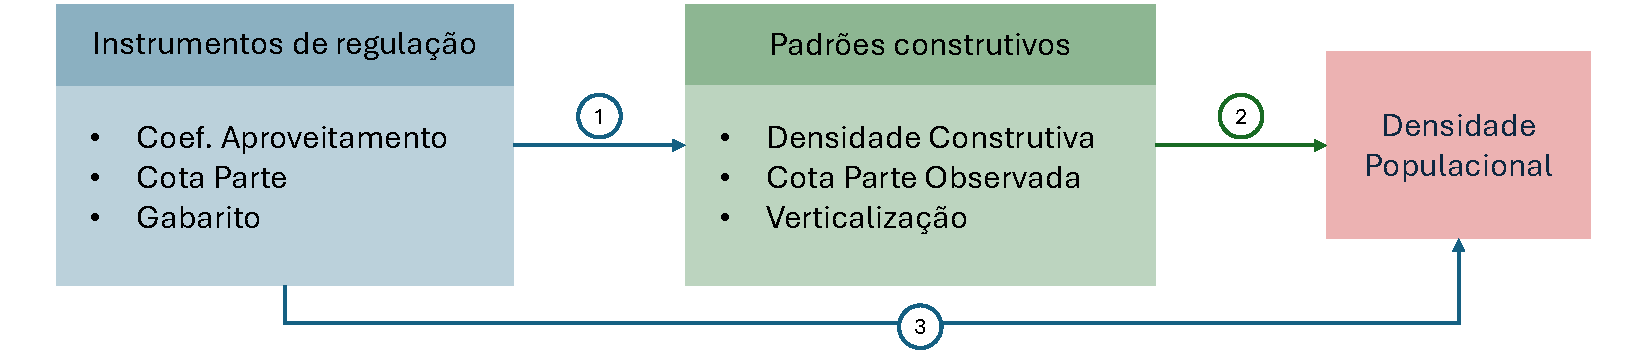
\includegraphics[width = \linewidth]{figuras/desenho_proposta.pdf}
    \label{fig:diagrama}
\end{figure}

\subsection*{A regulação foi capaz de influenciar os padrões construtivos na cidade da maneira esperada?} 

Através dos instrumentos apresentados na Seção \ref{sec:plano-diretor}, o PDE pretendia que o desenvolvimento imobiliário se concentrasse na Macrozona de Estruturação e Qualificação Urbana, em especial nos EETUs, que receberam um novo conjunto de regras. Em grande parte, essas mudanças permitiram um adensamento construtivo maior, verticalização ilimitada e impuseram uma densidade habitacional mínima. Todavia, como mencionado na Seção \ref{sec:motivacao}, a cidade é composta de diversos interesses, sendo o mercado imobiliário um agente central nesse aspecto. 

O mercado imobiliário, responsável por de fato construir novas habitações, responde à regulação sempre buscando maximizar seu lucro. Como a regulação não criou incentivos e na verdade, apenas mudou permissões em cada região da cidade, não necessariamente o mercado imobiliário aceita o novo conjunto de regras como um convite para construir a tipologia que o PDE deseja ver nos EETUs. Dentro dos limites da legislação de CA entre 2 e 4, há muita liberdade para o mercado escolher o que construir. Ademais, sempre existe a opção de não construir nessas regiões, quando o benefício do maior potencial construtivo não é suficiente para compensar a taxação advinda da extrapolação do CA básico. 

\subsection*{Os padrões construtivos regulamentados e incentivados são de fato capazes de gerar a densidade esperada?} 

Em outras palavras, é possível afirmar que maior densidade construtiva, mais verticalização e mais densidade habitacional se traduzem em maior densidade populacional? Embora a pergunta seja simples, há nuances a considerar. Primeiro, é essencial determinar se esses três componentes do padrão construtivo são relevantes e qual deles exerce maior influência sobre a densidade populacional.

Se a densidade construtiva for um fator determinante da densidade populacional, o instrumento do CA assume importância. De forma semelhante, se a densidade habitacional ou a verticalização tiverem maior destaque, a cota parte e o gabarito tornam-se relevantes. Assim, responder a esta questão ajuda a identificar quais dos instrumentos analisados na pergunta 1 são mais significativos.

\subsection*{A regulação foi capaz de influenciar a densidade populacional na cidade?} 

O PDE propôs uma relação causal, ilustrada na Figura \ref{fig:diagrama}, que pressupõe que, se as duas primeiras condições forem atendidas, o aumento da densidade populacional será uma consequência direta. Ou seja, a terceira pergunta se tornaria desnecessária caso as duas primeiras se confirmassem.

Contudo, essa relação não é garantida, pois outros fatores também podem influenciar a densidade populacional, independentemente das regulamentações introduzidas. Assim, é essencial avaliar o efeito total da regulação sobre a densidade populacional, a fim de compreender o impacto completo e real das políticas implementadas.

\subsection*{Direcionamento no artigo}

No Capítulo \ref{chp:revisao} é feita uma breve revisão literária. No Capítulo \ref{chp:dados} serão apresentados os dados utilizado nas análises. No Capítulo \ref{chp:analise} será discutida a metodologia e resultados para cada uma das perguntas. No Capítulo \ref{chp:conclusao} serão trazidas as reflexões finais, na Seção \ref{sec:conclusao} o foco é nos principais resultados, e na \ref{sec:contribuicoes} é feita uma discussão com implicação mais direta no debate público. Por fim, nos Apêndices há discussões de detalhes importantes, mas que tangenciam a narrativa do trabalho.

Os códigos utilizados para gerar os resultados apresentados estão disponíveis de maneira pública para verificação, replicação ou utilização para outros fins, contato que este trabalho seja citado de maneira adequada\footnote{O código pode ser acessado na página do GitHub \href{https://github.com/gustavo-tm}{neste link.}}.


\chapter{Revisão Literária}
\label{chp:revisao}

\section{O papel da regulamentação}

Na literatura microeconômica há diversos modelos que tentam compreender as dinâmicas econômicas da cidade, analisando como as forças de mercado agem na ausência da regulação. Utilizando premissas formais e provas matemáticas, é possível resolver os modelos para algumas variáveis endógenas, como preço por metro quadrado na cidade, uso do solo, densidade populacional, entre outros. O que geralmente há de comum entre estes modelos, é que se o mercado receber um tratamento \textit{laissez-faire}\footnote{O tratamento \textit{laissez-faire} se refere à pouca influência do governo nas decisões dos agentes econômicos}, se observará um maior adensamento no centro, onde há oferta de emprego. Quando há múltiplos centros, ou pontos de transporte público de alta capacidade, também há maior adensamento no entorno deles \cite{papageorgiou2012essay, fujita1989urban}.


Isso acontece porque o adensamento traz diversos benefícios econômicos. A aglomeração tecnológica $(i)$ aumenta a produtividade dos trabalhadores, na medida em que os empregos são mais concentrados e há ``transbordamento'' de conhecimento entre as firmas da região. Além disso, uma oferta maior e mais diversa de trabalho, causa maior competitividade e eficiência na escolha da pessoa certa para cada cargo. Aglomerações pecuniárias $(ii)$ reduzem os custos das firmas, sem alterar sua produtividade. Com maior demanda por serviços como segurança, limpeza, contratação e advocacia, estes mercados se desenvolvem, tornam-se mais competitivos, eficientes e baratos. Inclusive, há serviços especializados de nicho, que podem estar disponíveis e acessíveis apenas em grandes centros urbanos. Aglomeração de varejo $(iii)$ traz ganhos para os consumidores e comerciantes. Quando o comércio está aglomerado, o consumidor pode escolher entre mais opções e se desloca menos entre seus destinos caso queria comprar mais de um item. Dessa forma, os consumidores ganham e os comerciantes também, visto que com mais consumidores e maior fluxo, maiores as vendas. Por fim, o custo de transporte $(iv)$ é um dos fatores que mais mudam quando há densidade. A redução do custo de transporte, que pode ser considerada uma economia de aglomeração pecuniária, acontece não apenas para os trabalhadores, que se deslocam menos às oportunidades de emprego, mas também às firmas que gastam menos transportando seus bens e serviços \cite{brueckner2011lectures}.

Entretanto, ao introduzir falhas de mercado nesses modelos, a organização da cidade na ausência de regulamentação pode estar associada cenários não desejáveis. Muitas vezes estas falhas de mercado encadeiam uma expansão da mancha urbana, com implicações negativas no meio ambiente, além da perda dos benefícios da aglomeração. Um exemplo de falha de mercado está relacionada ao tráfego de carros. Este meio de transporte individual motorizado diminui os custos de viagens longas, possibilitando que os cidadãos habitem residências mais distantes de seus destinos. Todavia, além de causar uma expansão da mancha urbana, introduzir risco de acidentes e emitir poluentes, cada carro a mais que está na rua torna a viagem de todas as outras pessoas um pouco mais lenta. Apesar desses malefícios serem negligenciáveis nas escolhas individuais de utilizar ou não o carro, ou seja, um indivíduo racional não vai deixar de usar o carro, em uma cidade com milhões de habitantes, o custo individual negligenciado de cada carro se soma, de forma a ter um impacto significativo para a sociedade.

Nesse sentido, o governo poderia intervir, de forma a corrigir estas falhas de mercado, por exemplo, introduzindo um pedágio urbano. Dessa forma, seriam internalizadas as externalidades negativas dessa escolha individual de usar o carro. Com o dinheiro coletado desse imposto, poderiam ser compensados os danos causados, através de investimentos públicos. Entretanto, tal medida é difícil de ser implementada, levando os tomadores de decisão a tomar outro caminho no combate às externalidades. Regular os padrões construtivos pode ser uma forma alternativa de lidar com o problema, impedindo que as externalidades aconteçam. Nessa frente, o CA é um instrumento amplamente utilizado para regular o padrão construtivos e consta no plano diretor de cidades modernas nos Estados Unidos, Canadá, Alemanha, França, etc.

\begin{figure}[h]
    \caption{Impacto da regulação no CA da cidade}
    \centering
    \begin{subfigure}{.6\linewidth}
        \begin{tikzpicture}

    \begin{axis}[standard,
        xtick={0},
        ytick={.5},
        xticklabels = {},
        yticklabels = {$FAR_{reg}$},
        samples=100,
        xlabel={Distance to center ($x$)},
        ylabel={FAR},
        xmin=0,xmax=2,
        ymin=.2,ymax=1,
        y label style={anchor=east},
        x label style={anchor=north},
        clip=false
    ]
    
\addplot[domain={0:2}]{.8*e^(-.9*x)+.1} node[pos=1] (point1) {};
\node [right] at (point1) {\textit{laissez-faire}};

\addplot[domain={(ln(4.8)/1.3):2}]{1.2*e^(-1.3*x)+.25} node[pos=1] (point2) {};
\node [right] at (point2) {regulado};

\addplot[domain={0:(ln(4.8)/1.3)}]{.5};

\addplot[black, dashed] coordinates {((ln(4.8)/1.3),0) ((ln(4.8)/1.3),.5)};

\end{axis}
\end{tikzpicture}
    \end{subfigure}
    \label{fig:FAR}
\end{figure}

Caso o CA máximo regulado seja maior do que o mercado demanda, o CA observado será inferior ao limite, ou seja, a regulação não impacta essa região diretamente. Nas regiões em que a demanda por habitação é maior do que o permitido, parte da demanda precisam ser remanejada territorialmente, para que o limite não seja ultrapassado. No caso do PDE de 2014, a ideia é limitar o adensamento nas regiões periféricas e de proteção ambiental, direcionando o adensamento para as regiões centrais. Entretanto, caso o excesso de demanda esteja em uma área central, haverá um espraiamento para as periferias, causando o efeito contrário do estipulado. Na Figura \ref{fig:FAR} é possível observar um exemplo de CA máximo na cidade como um todo e a demanda por habitação excedente no centro, que com o limite máximo no CA, se dispersa em territórios mais distantes.


Portanto, caso o planejador central identifique incorretamente a demanda de mercado em cada região da cidade, é possível que a demanda reprimida encadeie um processo de expansão da mancha urbana e todas as externalidades negativas discutidas anteriormente. Além disso, quando a regulação é muito restritiva, há um incentivo indireto para que se desenvolva um mercado informal. Nesse sentido o CA, apesar de ser uma ferramenta poderosa no arsenal do planejador urbano, ela também é perigosa, visto que pode levar a efeitos adversos. 

\section{Evidências do PDE de 2014}

A literatura sobre o impacto do Plano Diretor Estratégico (PDE) de São Paulo, especialmente no que se refere ao aumento da densidade nas proximidades de transporte público, é limitada, com pouca produção quantitativa focada em inferência causal. A maior parte dos estudos existentes tem um perfil descritivo ou de discussão, observando os efeitos sem estabelecer relações causais claras. A revisão do PDE entre 2021 e 2023 gerou uma série de publicações, muitas delas descritivas, que discutem as mudanças introduzidas, mas ainda há uma lacuna em estudos que utilizem métodos quantitativos para avaliar o impacto real dessas políticas.

Durante o período de revisão do PDE, diversas notas técnicas foram importantes para as discussões que estavam ocorrendo. Houve evidências que apontavam para um adensamento construtivo nas regiões dos eixos, ainda que houvesse heterogeneidade espacial \cite{IU50, nt1, nt2, Marques2023}. Algumas estatísticas também foram feitas para analisar a atividade econômica e emprego formal \cite{IU52, IU54}. 

O principal estudo que se destaca por apresentar inferência causal para o aumento do adensamento construtivo foi intitulado ``Estimating the economic value of zoning reform''. O artigo, mostra que nas regiões em que houve um aumento no CA máximo, pode-se observar um aumento na densidade construtiva em relação às que mantiveram o mesmo, ou reduziram o CA máximo \cite{Anagol2021}.

Entretanto, há uma lacuna na literatura para a identificação do efeito do PDE sobre a densidade populacional. As estatísticas descritivas geradas foram em grande parte inconclusivas sobre a efetividade do PDE \cite{IU51, IU66}. Ainda, no documento divulgado em 2021 com o diagnóstico dos desdobramentos do PDE feito pela Secretaria Municipal de Urbanismo e Licenciamento da prefeitura de SP, destaca-se a seguinte conclusão da efetividade dos eixos: ``após as análises realizadas pelo monitoramento é possível verificar que houve grande adensamento construtivo em algumas áreas da cidade, porém ainda não há condições de aferir
o adensamento populacional'' \cite{PDE:diagnostico}.

\chapter{Dados}
\label{chp:dados}

\section{Padrões Construtivos}
\label{sec:dadosIPTU}

Em relação aos dados sobre os empreendimentos imobiliários, a base de dados escolhida foi do IPTU. Para os fins deste artigo, ela é a mais completa, visto que não representa um fluxo de novos imóveis construídos todos os anos como a base da Embraesp, mas apresenta um estoque imobiliário de tudo que já foi construído de moradia formal na cidade. Dito isso, estão cadastrados os 3.096.719 números únicos de contribuintes, que, segundo a definição da documentação dos dados no GeoSampa, ``A cada imóvel urbano corresponderá um número de inscrição no Cadastro Imobiliário Fiscal, entendendo-se como imóvel: I - a área de terreno, construído ou não, definida em matrícula do competente Serviço de Registro de Imóveis ou em transcrições ainda vigente''. Os únicos dados que não constam nessa base são relativos a lotes irregulares ou não registrados -- este tópico será discutido adiante.

Entre os dados disponíveis do IPTU, se destacam a área do terreno, a área construída, a área ocupada, o tipo de uso e o número de pavimentos do empreendimento. Logo, com estes dados é possível identificar os padrões construtivos na cidade, mantendo os cálculos os mais fiéis possível à forma como são calculados pela regulação. A densidade construtiva, por exemplo, é definida pelo CA observado no lote. 

\begin{figure}[h]
    \centering
    \caption{Distribuição do padrão construtivo em cada lote residencial de São Paulo}
    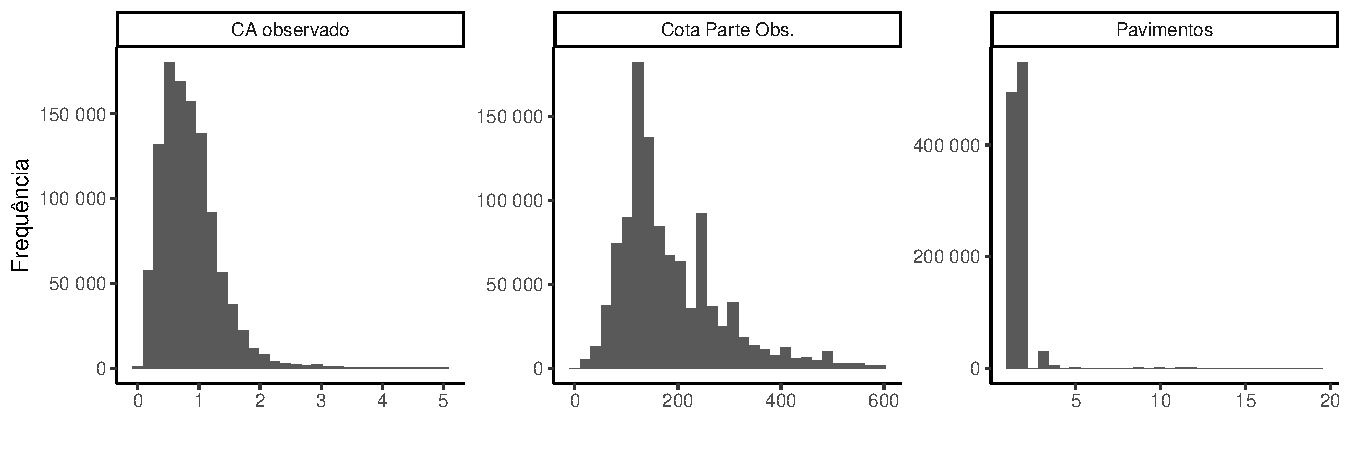
\includegraphics[width = \linewidth]{figuras/indicadores.pdf}
    \label{fig:histogramas}
\end{figure}

De fato, ao observar os indicadores na Figura \ref{fig:histogramas}, é possível notar que o perfil habitacional de São Paulo é bastante horizontal. É surpreendente que 95\% dos lotes residenciais formais em São Paulo apresentam 2 ou menos pavimentos. Ainda, a mediana do CA observado é 0,8, o que indica que em mais da metade dos lotes da cidade foi construído menos do que a área do terreno. Ainda, a mediana da cota parte observada dos lotes da cidade é de 155$m^2$, o que representa um uso do terreno para poucas unidades habitacionais em média -- a mediana da cota parte observada é aproximadamente 8 vezes maior do que a cota parte máxima permitida nos EETUs. Apesar disso, estes indicadores a partir dos anos 2000 apresentaram uma tendência de adensamento e verticalização. Na Figura \ref{fig:indicadores-tempo} do Apêndice \ref{appendix:figuras} é possível observar a evolução dos padrões construtivos no tempo e na Figura \ref{fig:area_construida} está a distribuição da área construída dedicada a cada tipo de uso e perfil de densidade.

\section{Regulação}
\label{sec:dadosPDE}

Os dados da regulação são disponibilizados também de maneira pública no site da prefeitura junto ao PDE, mas pode também ser acessado pelo GeoSampa. O principal dado utilizado foi das áreas de influência dos ativadores de eixo, para que cada região pudesse ser classificada como dentro ou fora da zona de EETU.

\section{Densidade populacional}
\label{sec:dadosCenso}

Os dados de densidade populacional, são produzidos pelo Censo demográfico do IBGE, que ocorre a cada 10 anos. O Censo de 2020 se atrasou para 2022 por conta da pandemia e os dados começaram a ser divulgados em 2024. Até o momento, o que foi disponibilizado de maneira pública é a malha preliminar do Censo. Considerando que o PDE entrou em vigor em 2014, foi utilizado o Censo de 2010 como um período pré PDE e o Censo de 2022 como período pós. Segundo o levantamento de 2022, a atual população do município de SP se encontra em 11.451.999 de habitantes, divididos em 4.996.529 de domicílios, dos quais apenas 4.316.336 estão ocupados. Na Figura \ref{fig:populacao} é possível observar quais são as áreas mais densas da cidade. Entre elas, destaca-se o centro da cidade (Sé) e as favelas de Paraisópolis e Heliópolis.

\begin{figure}[!h]
    \centering
    \caption{Densidade populacional em São Paulo por setor censitário (Censo 2022)}
    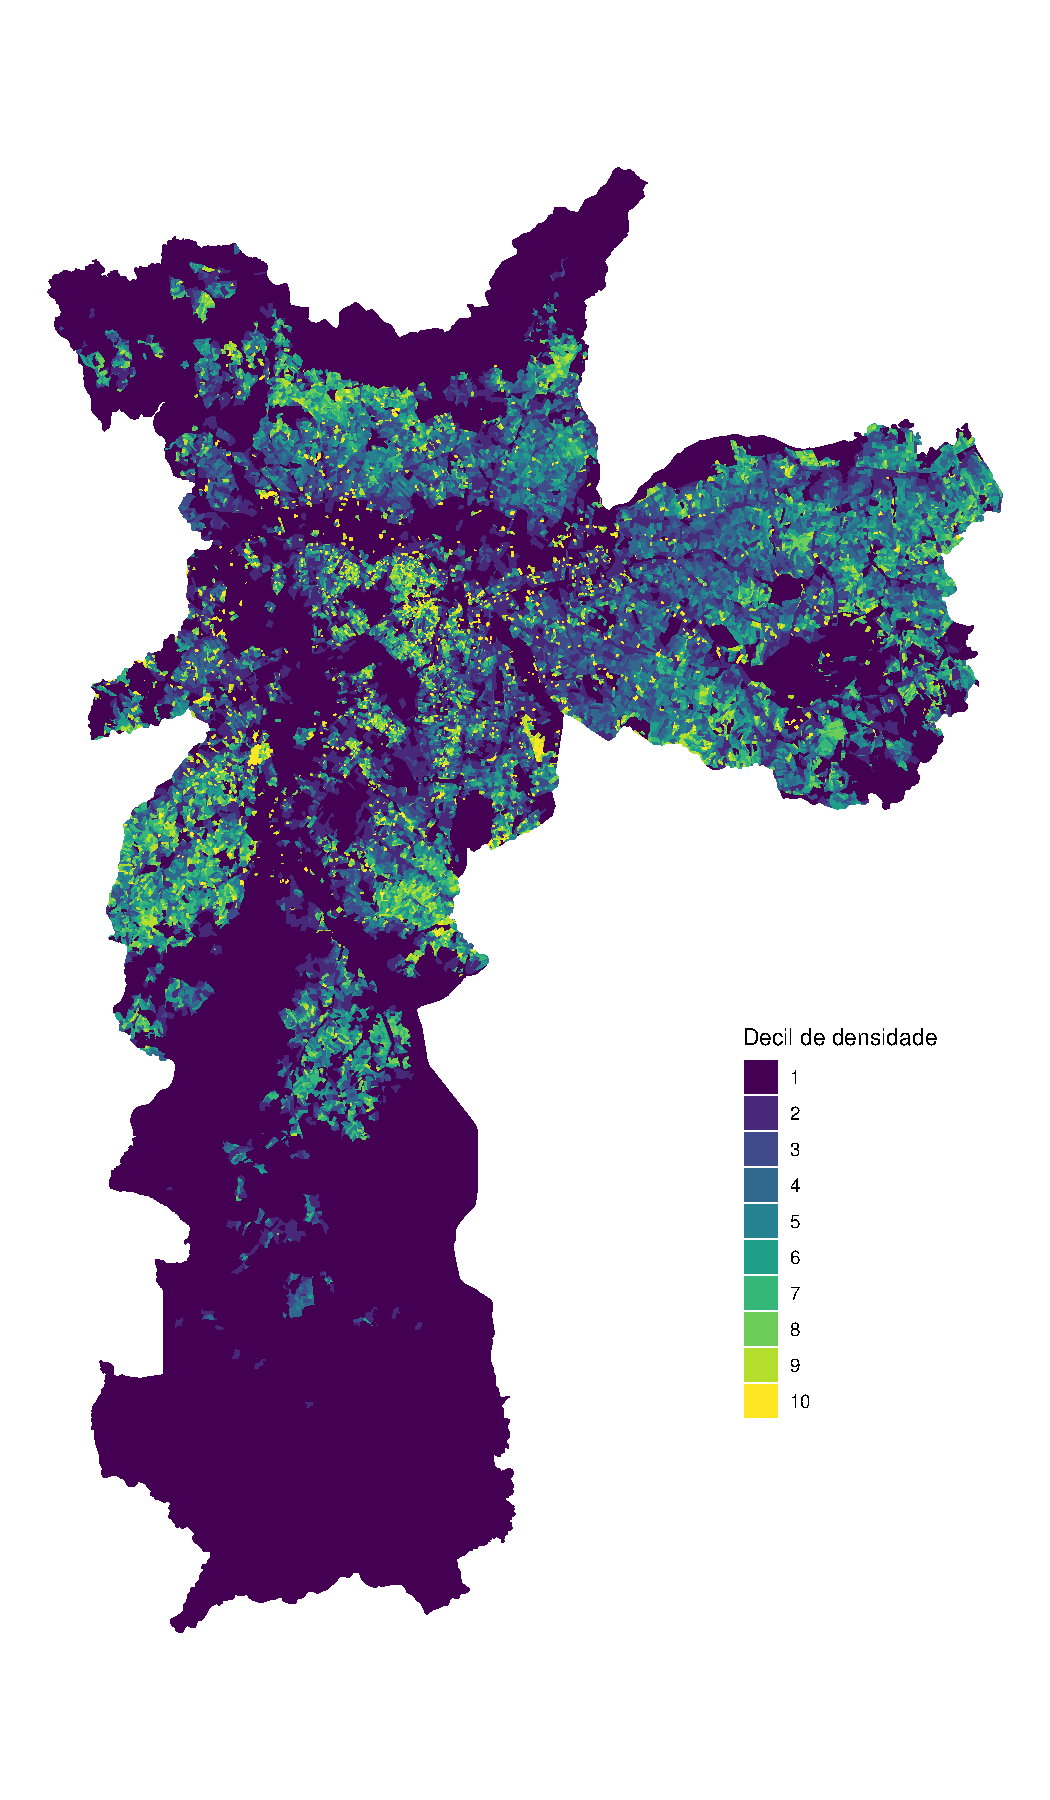
\includegraphics[width = .95\linewidth]{figuras/mapa-densidade.pdf}
    \label{fig:populacao}
\end{figure}

A unidade de observação do censo mais próxima de microdados que pode ser georreferenciada é o setor censitário\footnote{Para estar em conformidade com a Lei Geral de Proteção de Dados (LGPD), é importante proteger a anonimidade dos entrevistados, então deve haver algum tipo de agregação geográfica.}. Os limites dos setores são construídos de forma que o agente de coleta do censo consiga cobrir o setor inteiro, minimizando os erros de medição e otimizando o processo. A metodologia para a delimitação dos setores censitários leva em consideração diversos fatores, como elementos na paisagem que se constituam em barreiras naturais ou artificiais e dificultam o trabalho do agente, pontos de referência estáveis e de fácil identificação no terreno, limites das estruturas territoriais como bairros e quadras, entre outros \cite{IBGE2024}. Um fator determinante para o tamanho do setor censitário é o número de domicílios a serem entrevistados, que em áreas urbanizadas deve estar entre 250 e 400 para os mais densos e entre 150 e 250 para os menos densos.

\clearpage
\section{Cruzamento dos dados}
\label{sec:dadosCruz}

Parte da dificuldade de discutir os temas urbanos com dados é a complexidade de trabalhar com eles. Como é possível observar na Tabela \ref{tab:dados}, cada base de dados apresenta um nível de observação e frequência diferente. Portanto, sempre é necessário que haja alguma agregação territorial e/ou temporal para que a análise seja possível. Como comentado anteriormente, a metodologia de processamento de dados utilizada neste artigo está disponível em um repositório público.

\begin{table}[h!]
    \centering
    \caption{Information about each database}

    {\small
    \begin{tabular}{>{\raggedright\arraybackslash}p{0.125\linewidth} >{\raggedright\arraybackslash}p{0.50\linewidth} >{\centering\arraybackslash}p{0.125\linewidth} >{\raggedright\arraybackslash}p{0.15\linewidth}}
        % \toprule
        \textbf{Data} & \textbf{Source} & \textbf{Frequency} & \textbf{Scale} \\
        \midrule
        Census & Brazilian Institute of Geography and Statistics (IBGE) & Decennial & Census tract \\
        Property Tax (IPTU) & Property Tax and Maintenance Registry maintained by the Municipal Department of Finance (DECAD) of São Paulo's City Hall & Annual & Taxpayer \\
        Plots & Fiscal Real Estate Registry of the Municipal Department of Finance & Annual & Plot \\
        Regulation & Department of Urbanism and Licensing (SMUL) & 2014 & Zone perimeter \\
        \bottomrule
    \end{tabular}
    }
    \label{tab:datasets}
\end{table}


Os dados do IPTU não são georreferenciados, então desacompanhados de outros dados não é possível cruzá-los com os do Censo. O que possibilita fazer essa junção é que o número único de contribuinte do IPTU, também é o código do Setor, Quadra e Lote (SQL) que o empreendimento se encontra. Nesse sentido, é possível decompor o SQL e cruzar com as bases de lotes, que contêm a geometria de cada  um dos 1.677.980 lotes da cidade. O que explica a diferença entre o número de lotes e número de números dos contribuintes são os lotes que contém um condomínio, que pode haver diversos números únicos de contribuintes em apenas um lote. Nos dados de IPTU, há 1.314.353 contribuintes em lotes com apenas uma unidade habitacional e 33.129 condomínios, que contêm 1.782.366 unidades. Ao cruzar o SQL do IPTU com a base de lotes, 44.319 contribuintes não encontram um par na outra base, o que representa uma perda de 1,67\% das unidades. 

Os dados da regulação não são codificados com o SQL, mas podem ser cruzados geograficamente. O perímetro de zona é um limite administrativo geralmente igual às quadras, mas pode ser um subespaço das quadras em alguns casos. Para determinar quais áreas são de EETUs, os perímetros de zona de eixo foram unidos e um contorno das regiões de EETU foi criado. O mapa com o resultado pode ser visto no Apêndice \ref{appendix:figuras}, Figura \ref{fig:eixos}. 

Como o perímetro de zona é bastante aderente à estrutura das quadras, a classificação dos lotes em estar dentro ou fora da região de eixo é direta. Por outro lado, os setores censitários seguem uma estrutura completamente diferente. Há vezes que um setor censitário contém diversos lotes, mas é possível que um lote contenha também mais de um setor censitário. Para fins práticos, os dados do IPTU, censo e regulação foram cruzados geograficamente. Uma discussão com maior detalhamento pode ser consultada no Apêndice \ref{appendix:cruzamento}.

Os setores censitários são uma partição\footnote{Uma partição é uma divisão que ocupa o espaço por completo, sem que haja intersecção entre os elementos.} do espaço da cidade de São Paulo, o que implica que a área do setor censitário é composta não apenas pelos lotes, mas também por trechos que contém ruas, parques, usos não residenciais, entre outros fatores. Na Figura \ref{fig:area-setor} é possível identificar que apenas um terço da área do setor censitário é dedicado ao uso residencial. Além disso, no raio de 1km dos eixos, aproximadamente 4\% dos empreendimentos residenciais foram construídos após PDE\footnote{Este valor está superestimado, visto que grande parte dos prédios que ficaram prontos entre 2014 a 2017 foram aprovados durante a vigência do PDE de 2002.}.
 
\begin{figure}[h]
    \centering
    \caption{Dedicação do espaço do setor censitário para cada uso em um raio de 1km dos eixos}
    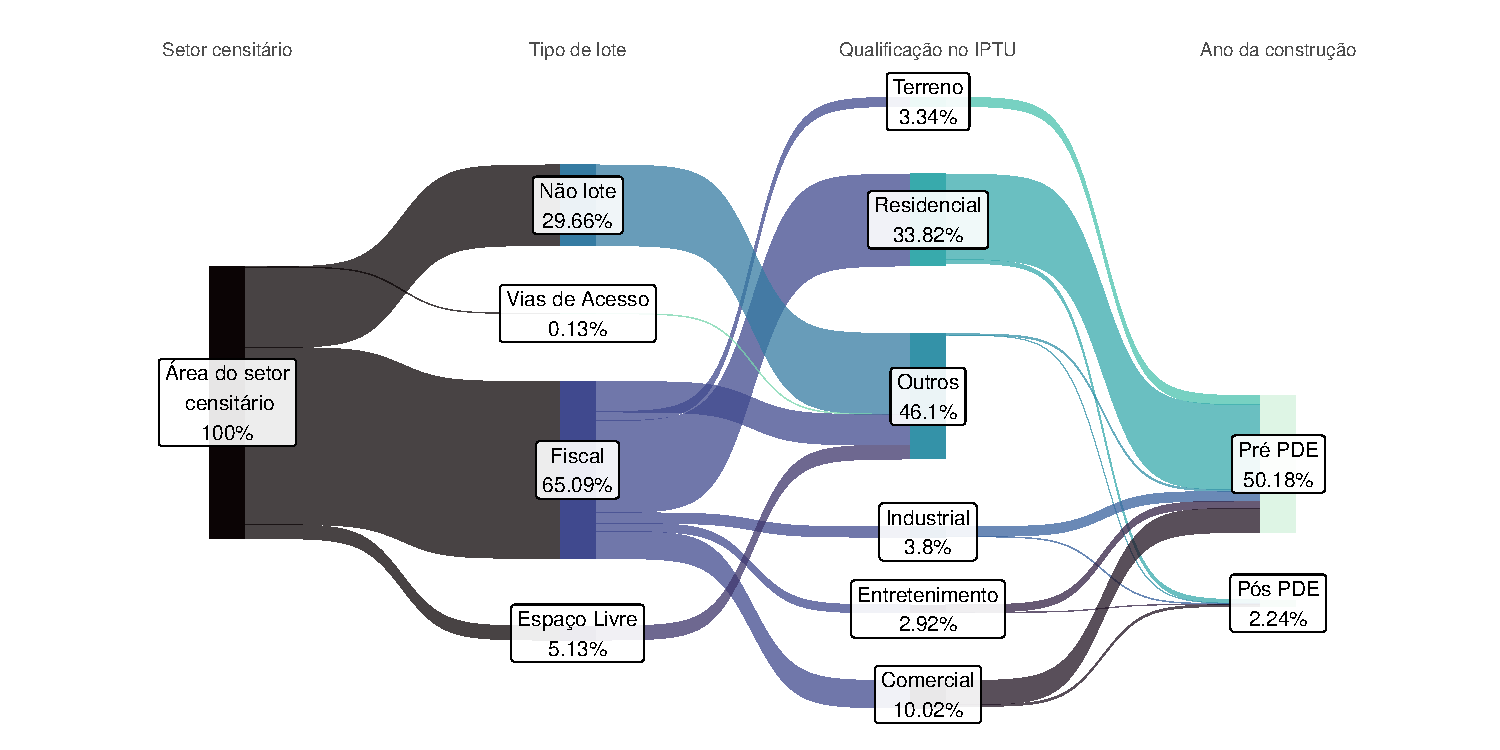
\includegraphics[width = \linewidth]{figuras/area_setor.pdf}
    \label{fig:area-setor}
\end{figure}

Uma oportunidade ao integrar esses dados é validar informações comuns a ambos. O número de moradias, por exemplo, está disponível tanto nos registros do IPTU quanto no Censo. Essa comparação possibilita avaliar o nível de moradia informal em cada região, já que o Censo oferece dados mais abrangentes e confiáveis nesse aspecto. Assim, uma moradia registrada no Censo, mas ausente no IPTU, pode ser considerada informal. Em termos quantitativos, dos 4.996.529 domicílios contabilizados pelo Censo, apenas 2.641.635 estão registrados no IPTU, o que indica um índice de regularidade habitacional (legal) de aproximadamente 52,87\%. Mais detalhes sobre a informalidade são discutidos no Apêndice \ref{appendix:informalidade}, mas é importante destacar que os resultados desta pesquisa se aplicam exclusivamente às moradias formais.

\chapter{Metodologia e Resultados}
\label{chp:analise}

Como comentado na Seção \ref{sec:problema}, há três perguntas a ser respondidas, que podem ser visualizadas no diagrama da Figura \ref{fig:diagrama}. Nas seções a seguir, cada uma das perguntas será respondida através da análise quantitativa dos dados apresentados.


\section{Do padrão construtivo à densidade populacional}
\label{sec:perg1}


O objetivo desta seção é responder: \textbf{Os padrões construtivos regulamentados e incentivados são de fato capazes de gerar a densidade esperada?} Para tanto, foram considerados os dados do Censo de 2022 e os do IPTU do mesmo ano. Para esta seção, a regulação de cada região da cidade não é importante, visto que o foco é em identificar qual a relação entre a densidade construtiva, densidade habitacional e pavimentos com a densidade populacional e esta relação não é modificada pelo PDE. A influência do PDE recai sobre estes três componentes do padrão construtivo, através da regulação do CA, cota parte e gabarito, respectivamente. Dessa forma, validar a importância desses padrões construtivos significa validar também os instrumentos de regulação.

Para inferir a relação entre as 3 variáveis e a densidade populacional, foram adotadas duas abordagens complementares e cada uma tem seus pontos fortes e fracos: regressão linear e \textit{random forest}. A principal diferença entre as abordagens é que a regressão, por estar no universo da econometria, apresenta maior interpretabilidade, mas também requer algumas suposições para apresentar validade. A \textit{random forest}, por pertencer ao mundo do \textit{machine learning}, tem a característica de ser mais difícil de interpretar, sendo considerada muitas vezes um modelo \textit{black box} (caixa preta). Por outro lado, enquanto a regressão linear exige uma forma funcional fundamentada economicamente, a \textit{random forest} encontra as relações não necessariamente linear entre as variáveis do modelo por conta própria. No caso desta seção da pesquisa, os regressores do da densidade populacional são instrumentos de regulação e não fatores econômicos discutidos na Seção \ref{chp:revisao} como distância ao centro, dificultando a plausibilidade de suas exogeneidades.

% A primeira foi de utilizar uma regressão linear, que apresenta maior interpretabilidade, mas a principal limitação dessa abordagem é que a forma funcional da regressão no contexto desta pesquisa não está fundamentada economicamente, o que a torna sujeita a problemas de endogeneidade, e, portanto, enfraquece a validade da inferência. A abordagem alternativa, de árvores de regressão, transita do universo da econometria para o universo do \textit{machine learning}. Apesar de ter uma interpretabilidade mais restrita, as árvores de regressão não precisam de uma forma funcional como a regressão linear, mas conseguem encontrar relações não lineares entre as variáveis do modelo.

O primeiro passo para implementar estas metodologias consiste em combinar as bases de dados em um nível de observação único. Para manter os dados na escala mais desagregada possível, os dados poderiam ser combinados geograficamente ao nível do setor censitário. Porém, como foi discutido na Seção \ref{sec:dadosCenso}, o tamanho do setor censitário depende diretamente tanto da população que o habita, quanto de sua densidade, o que traria viés para a regressão\footnote{Neste caso, a densidade populacional depende da área do setor censitário, que não pode ser omitida da regressão. Entretanto, se for utilizada como um regressor, apresentará uma relação de simultaneidade com a variável dependente, já que quanto mais densa uma região é, menor será sua área. Sendo assim, seria necessário fazer uma estimação por equações simultâneas, trazendo complexidade para a identificação, já que não há variáveis exógenas suficientes para recuperar os parâmetros de interesse}. Desse modo, o mapa da cidade foi recortado em um \textit{raster} (quadriculado) com células de 800m de largura e os dados tanto do censo quanto do IPTU foram agregados nessa escala. Os detalhes mais técnicos podem ser encontrados no Apêndice \ref{appendix:cruzamento}. 

Por fim, foram selecionadas apenas as células do raster que apresentavam um baixo grau de informalidade. O espectro de irregularidade foi calculado comparando o número de domicílios registrados no Censo com o total de unidades registradas no IPTU. Quando uma região se encontra no extremo esquerdo do espectro (próximo de 0\%), isso indica que, embora haja domicílios registrados no Censo, a área não possui moradias formais. Valores próximos a 50\% refletem equilíbrio entre os dados do Censo e do IPTU, indicando ausência de informalidade. Valores acima de 50\%, que representam um número maior de unidades no IPTU do que no Censo, são raros. Para mais detalhes sobre a informalidade, consulte o Apêndice \ref{appendix:informalidade}. 

\subsection{Abordagem de regressão linear}

{\tiny
\begin{table}[h]
\caption{Regression results for raster cells that present irregularity spectrum between 45 and 55\% in 2022} 
\centering
\fontsize{10.0pt}{12pt}\selectfont
\begin{tabular*}{.9\linewidth}{@{\extracolsep{\fill}}lcccc}
\toprule
 & \multicolumn{2}{c}{y = Population} & \multicolumn{2}{c}{y = Density} \\ 
\cmidrule(lr){2-3} \cmidrule(lr){4-5}
  & (A) Linear & (B) Log & (C) Linear & (D) Log \\ 
\midrule\addlinespace[2.5pt]
Intercept & 2121.210*** & 7.814*** & 6240.590*** & 8.583*** \\ 
Dwellings & 1.476*** & 0.000*** &  &  \\ 
Built area (m2) & 0.000 & 0.000+ &  &  \\ 
Verticalization & -131.656*** & -0.036** & 24.817 & -0.033 \\ 
Built Density &  &  & 705.142 & 0.199** \\ 
{Dwelling Unit Density} & {} & {} & {0.187***} & {0.000*} \\ 
\midrule
Num.Obs. & 332 & 332 & 332 & 332 \\ 
R2 & 0.861 & 0.602 & 0.319 & 0.223 \\ 
R2 Adj. & 0.860 & 0.598 & 0.313 & 0.216 \\ 
\bottomrule\vspace{0pt}
\end{tabular*}
\label{tab:regressao-1}
\begin{minipage}{.9\linewidth}
+ p < 0.1, * p < 0.05, ** p < 0.01, *** p < 0.001\\
\end{minipage}
\end{table}


}

Na Tabela \ref{tab:regressao-1} é possível observar os resultados de quatro regressões, todas com o mesmo intuito, porém com formas funcionais diferentes. Nas primeiras duas colunas, a população é regredida em unidades, metros quadrados de área construída e um indicador de verticalização. Interpretando a primeira coluna (A), é possível inferir que caso se mantenham constantes os outros componentes, uma unidade habitacional a mais está associada a 1,47 moradores a mais na região. O número de metros quadrados construídos não apresenta significância significância estatística. O coeficiente da verticalização indica que um aumento de 1 na verticalização\footnote{Um aumento de 1 na verticalização implicaria que todas as construções na célula do \textit{raster} tivessem um pavimento a mais} em média está associado a 130 pessoas a menos na célula do \textit{raster}. Para ter um parâmetro de comparação, a média da população por célula é de 4.600 habitantes, com uma dispersão considerável. A distribuição da população dos \textit{rasters} pode ser vista na Figura \ref{fig:populacao-rasters} do Apêndice \ref{appendix:figuras}. 

Na segunda coluna da tabela (B),  os resultados são semelhantes, mas a área construída passa a ser estatisticamente significativo e positivo, mas negligenciável. O coeficiente associado à verticalização continua negativo, indicando que é esperado que um aumento de 1 na verticalização esteja associado a 3,6\% menos pessoas habitando a região, caso todos os outros componentes continuem constantes. Nas colunas C e D da Tabela \ref{tab:regressao-1}, apesar das variáveis dependente e explicativas serem referentes a densidade\footnote{A densidade construtiva é calculada igual o CA (área construída / área do terreno) e a densidade habitacional é o inverso da cota parte (número de unidades / área do terreno)} e não valores absolutos, os resultados permanecem parecidos. A principal diferença é que a verticalização ao invés de ter uma relação inversa com a densidade, passa a ser estatisticamente irrelevante.

Apesar de contraintuitivo, o resultado apresenta uma interpretação razoável. O modelo econométrico (Coluna A) aponta que em cada unidade habitacional há em média 1,47 habitantes, mas caso estas mesmas unidades ganhem metragem de área construída é possível observar mais habitantes nestes domicílios, visto que se tornam mais espaçosos. O resultado associado à verticalização pode indicar que o perfil dos núcleos domiciliares que habitam imóveis mais verticalizados é de famílias menores. Outro resultado surpreendente é o intercepto. De maneira intuitiva, quando há zero pavimentos, nenhuma área construída e nenhuma unidade habitacional, a população deveria ser zero também, mas o modelo aponta para 2.121 pessoas. A explicação para isso são as moradias informais. Quando a regressão é feita para vários recortes do espectro de irregularidade, na medida em que o recorte se aproxima de selecionar apenas células equilibradas (espectro de irregularidade igual a 50\%), o intercepto se torna estatisticamente igual a zero. Em outras palavras, quando há irregularidade, o número de unidades é subestimado e o efeito é capturado pelo intercepto. A Figura \ref{fig:robustez-reg1} apresenta uma análise de robustez com todos os coeficientes e seus respectivos intervalos de confiança para cada intervalo de espectro de irregularidade selecionado.

\subsection{Abordagem de \textit{machine learning}}

Na abordagem de \textit{machine learning}, foi construído um modelo de \textit{random forest} \cite{wright2015ranger}. Uma das principais vantagens dessa técnica é que não exige a especificação de uma forma funcional, pois o próprio modelo seleciona as variáveis mais importantes e ajusta uma regressão não linear. Outro benefício da \textit{random forest} é sua capacidade de avaliar a importância relativa das variáveis, algo que não é diretamente testável em uma regressão linear.


Para desenvolver o modelo de floresta de regressão, a base de dados foi dividida em conjuntos de treino e teste, prevenindo \textit{overfitting}, ou seja, garantindo que o modelo aprenda padrões em vez de simplesmente memorizar os dados. Foram geradas 100 mil árvores com base nas células que apresentam um espectro de irregularidade entre 40\% e 60\%. Para avaliar a performance do modelo, foi replicada a regressão da Tabela \ref{tab:regressao-1} (Coluna C) com o método \textit{random forest}. Observou-se um $R^2$ de 81,9\% na base de teste, indicando um ganho significativo em poder explicativo. Esse ganho decorre exclusivamente da capacidade do modelo de capturar relações não lineares entre as variáveis, visto que os dados de entrada são os mesmos da regressão.

Para identificar quais variáveis são mais relevantes no modelo, foi aplicado um procedimento de permutação, no qual se introduz ruído nas variáveis explicativas para avaliar o impacto disso no erro do modelo \cite{breiman2001random, Nembrini2018}. Esse método permite quantificar a importância de cada variável para explicar a variável dependente. Como resultado, a \textit{random forest} identificou a densidade habitacional como a mais importante, seguida pela densidade construtiva e por fim a verticalização. Estes resultados são condizentes com os achados apresentados na Tabela \ref{tab:regressao-1}.

Com base na \textit{random forest} construída, também é possível simular a população de uma determinada região, com base em seus padrões construtivos. Para fins ilustrativos, foi considerada uma célula do raster, que possui largura de 800m. Nessa célula hipotética, a depender do CA, cota parte e verticalização observados, pode-se estimar a população que a habitaria. Na Figura \ref{fig:previsoes} é possível analisar os resultados. Em linha com que foi discutido até então, uma cota parte baixa parece ser o fator mais importante para obter uma densidade alta, principalmente se aliada à um CA alto. Um número maior de pavimentos, como já comentado, na maioria das situações está associado à uma densidade mais baixa ou igual, caso a densidade construtiva e habitacional se mantenha as mesmas.

\begin{figure}[h]
    \centering
    \caption{Simulações da \textit{random forest} para a população de uma célula hipotética de 800x800m}
    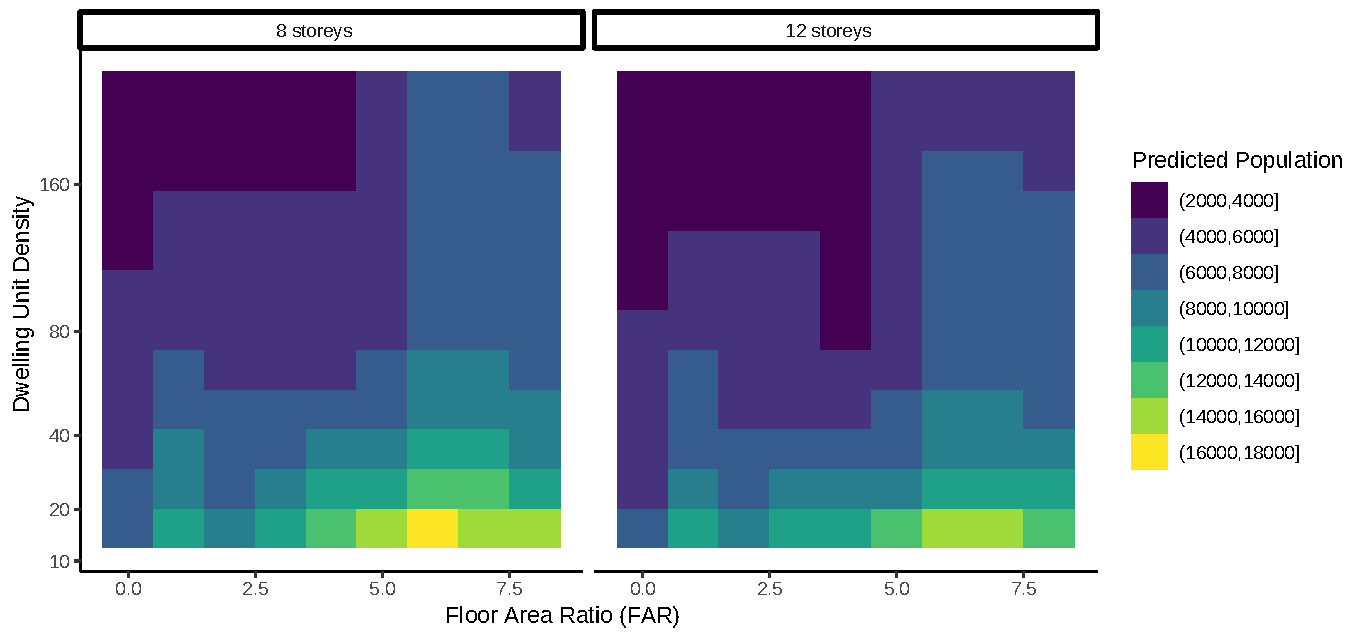
\includegraphics[width = \textwidth]{figuras/previsoes.pdf}
    \label{fig:previsoes}
\end{figure}

\subsection{Resultados principais}

Apesar das diferenças metodológicas, ambas as abordagens convergem para um resultado comum: a densidade habitacional é o componente do padrão construtivo mais importante para definir a densidade populacional. Esse achado é intuitivo, pois a quantidade de domicílios desempenha um papel central na determinação do número de habitantes. A densidade construtiva e o número de pavimentos, dados uma densidade habitacional e pavimentos constantes, podem ser vistos como modificadores do perfil desses domicílios.

Na medida que a densidade construtiva aumenta, as unidades habitacionais tendem a ser mais espaçosas, o que acomoda mais moradores em média. No caso da verticalização, com a densidade construtiva e habitacional fixas, qualquer aumento nos pavimentos exige uma redução na taxa de ocupação do terreno (conforme discutido na Seção \ref{sec:perg2} e no Apêndice \ref{appendix:verticalizacao}), resultando em edifícios com maiores recuos. Os dados sugerem que o mesmo número de unidades habitacionais e de área construída, quando inseridos em empreendimentos mais verticais, apresentam menos moradores em média. 

À luz dos resultados apresentados, a discussão sobre os instrumentos instituídos pelo PDE tomam um novo rumo. Os dados mostram que a verticalização, que foi incentivada nas zonas de eixos, não é uma aliada do adensamento, por vezes inclusive trabalhando no sentido contrário. O efeito da densidade construtiva foi em grande parte obstruído pelo potencial que a densidade habitacional tem de gerar densidade. Nesse sentido, se o PDE almeja definir quais regiões da cidade devem apresentar maior ou menor densidade, seria mais efetivo focar na cota parte e permitir um CA e gabarito suficientes para a construção das unidades habitacionais\footnote{Uma cota parte de 20 significa que, com o CA básico, cada unidade habitacional apresentará 20 metros quadrados. Estas mesmas unidades com um CA de 4 podem apresentar em média 80$m^2$. Todavia, é impossível atingir um CA 4 com menos de 4 pavimentos. Inclusive, quando há recuos obrigatórios, é necessário um número de pavimentos maior do que o CA para que seja possível construir todos os metros quadrados de área}.  

\clearpage
\section{Da regulação ao padrão construtivo}
\label{sec:perg2}

O objetivo desta seção é responder: \textbf{A regulação foi capaz de influenciar os padrões construtivos na cidade da maneira esperada?} Para tanto, foi escolhida também duas abordagens. Ambas são, em sua essência, metodologias de regressão em descontinuidade (RDD\footnote{Do inglês, \textit{Regression Discontinuity Design}}). Essa escolha é ideal por conta da exogeneidade na qual foi definido quais lotes pertenceriam ou não às áreas de eixo perto de sua fronteira. Como comentado na Seção \ref{sec:plano-diretor}, para se tornar uma zona de EETU, o lote deve estar dentro da área de influência do transporte coletivo de alta capacidade. Nesse sentido, os lotes vizinhos aos classificados como dentro da zona de eixo são um controle perfeito, visto que a diferença entre um lote de tratamento e o outro de controle é apenas atravessar a rua. Outras regiões da cidade também tiveram suas regulações alteradas, mas o foco da identificação 

\begin{figure}[h]
    \centering
    \caption{Exemplo de separação dos grupos de controle e tratamento na Vila Mariana}
    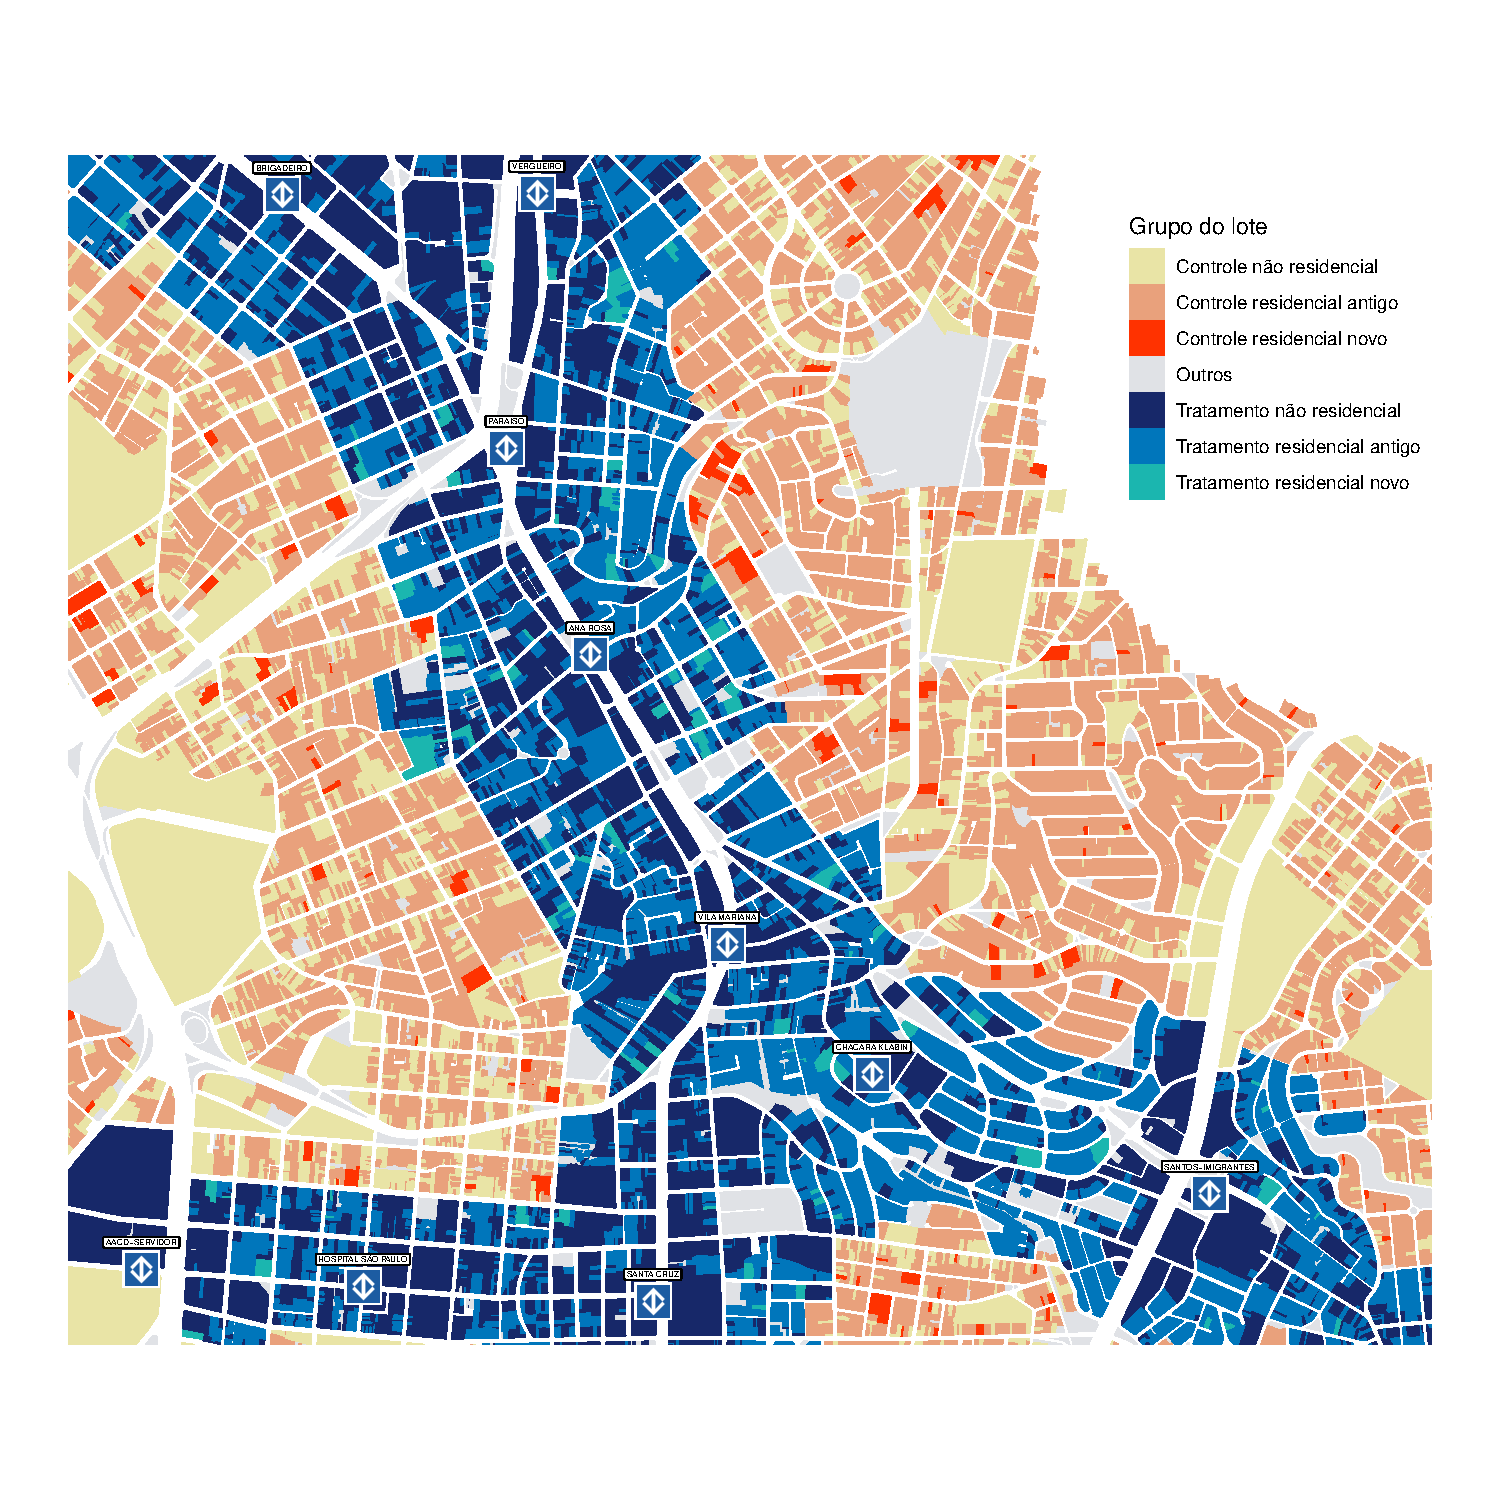
\includegraphics[width = .9\textwidth]{figuras/mapa-lotes-metro.pdf}
    \label{fig:mapaRDD}
\end{figure}

Na Figura \ref{fig:mapaRDD} é possível ver um exemplo de classificação dos lotes como controle e tratamento na Vila Mariana, região de eixos ativados por estações de metrô, em uma região de união de duas linhas, a verde e a azul. Um empreendimento é considerado novo caso ele tenha sido terminado de construir depois de 2014, ano de início da vigência do PDE. 

Antes de partir para a inferência causal, alguns resultados interessantes podem ser obtidos através da estatística descritiva. Primeiramente, não é possível observar uma grande diferença no número de lotes edificados entre o grupo controle e tratamento após 2014 na Figura \ref{fig:delta-IPTU-lotes}. No entanto, estes lotes passaram a apresentar um número maior de unidades habitacionais, como está ilustrado na Figura \ref{fig:delta-IPTU-lotes}. Isso é um indicativo de aumento da densidade habitacional.  

\begin{figure}[h]
    \centering
    \caption{Mudança no número de lotes edificados  na fronteira (50m) dos eixos}
    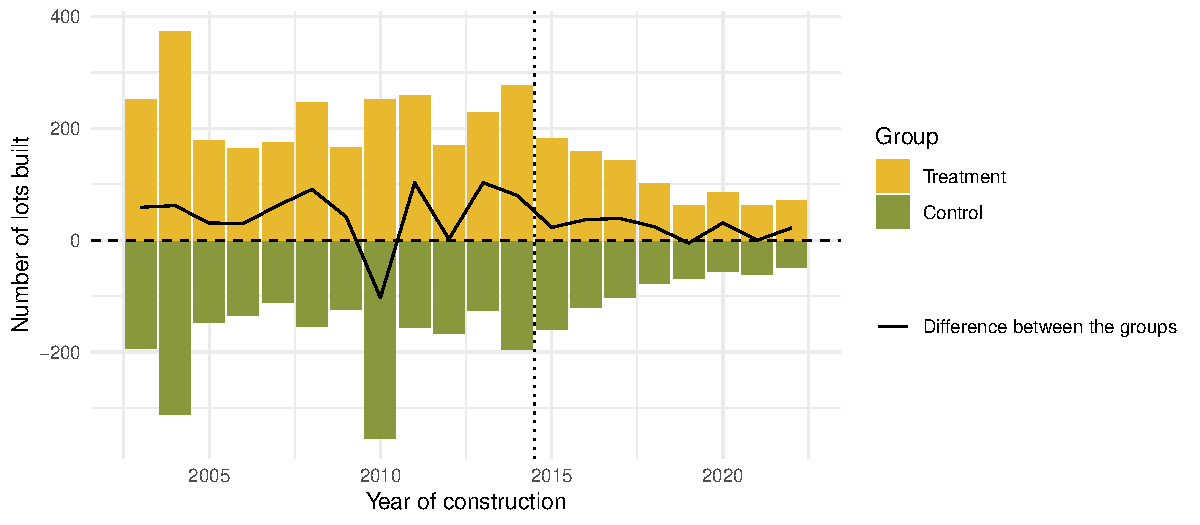
\includegraphics[width = .8\textwidth]{figuras/IPTU-delta-lotes.pdf}
    \label{fig:delta-IPTU-lotes}

    \caption{Mudança no número de moradias construídos na fronteira (50m) dos eixos}
    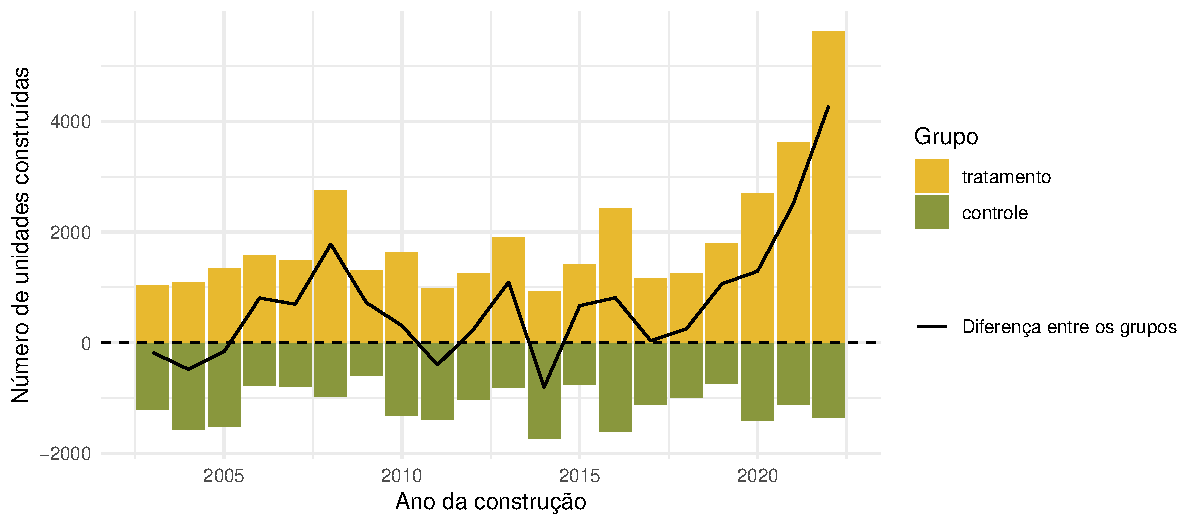
\includegraphics[width = .8\textwidth]{figuras/IPTU-delta-unidades.pdf}
    \label{fig:delta-IPTU-unidades}
\end{figure}

\subsection{Abordagem \textit{diff-in-diff} geográfico (e \textit{event study})}

O \textit{diff-in-diff (DiD)} geográfico é uma categoria de regressão de diferenças em diferenças que leva em consideração a proximidade espacial das observações para a definição dos critérios de controle e tratamento. Neste caso, foram definidos como tratamento todos os lotes residenciais que estão dentro da distância de 50m entre o centroide e a borda do eixo e como controle, a mesma distância, mas para os lotes que estão fora da zona de EETUs. A hipótese de identificação é igual a de um DiD comum: os grupos dois grupos, na ausência do tratamento, precisam apresentar tendências paralelas. 

\begin{table}[!t]
\caption{\label{tab:analise/did-IPTU}Resultados do DiD para unidades dentro de 50m da fronteira de eixo} 
\fontsize{12.0pt}{14.4pt}\selectfont
\begin{tabular*}{\linewidth}{@{\extracolsep{\fill}}lcccc}
\toprule
  & densidade\_construtiva & densidade\_habitacional & pavimentos & residencial \\ 
\midrule\addlinespace[2.5pt]
Intercepto & 1.031*** & 0.008*** & 1.992*** & 0.780*** \\ 
Tratamento & -0.001 & 0.000 & 0.027 & -0.011*** \\ 
Pós PDE & 0.891*** & 0.009*** & 1.661*** & -0.100*** \\ 
{Tratamento x Pós PDE} & {0.903***} & {0.011***} & {2.392***} & {0.001} \\ 
Num.Obs. & 59904 & 59904 & 59904 & 77625 \\ 
R2 & 0.027 & 0.032 & 0.026 & 0.001 \\ 
R2 Adj. & 0.027 & 0.032 & 0.026 & 0.001 \\ 
\bottomrule
\end{tabular*}
\begin{minipage}{\linewidth}
+ p < 0.1, * p < 0.05, ** p < 0.01, *** p < 0.001\\
\end{minipage}
\end{table}



A Tabela \ref{tab:did-IPTU} traz os resultados do DiD escolhendo cada componente do padrão construtivo como variável de interesse. Os dados apontam que a introdução dos eixos é responsável por aumentar em média a densidade construtiva em 0,9, a densidade habitacional em 0,011 domicílios por metro quadrado de terreno e 2,4 pavimentos. O eixo não altera a probabilidade do lote ser ou não residencial, como mostra a quarta coluna da regressão. Além disso, para este recorte de 50m, não há diferença estatisticamente significante entre os grupos de controle e tratamento antes do PDE. Os resultados são robustos às diferentes escolhas para o recorte de proximidade à borda. Na Figura \ref{fig:robustez-did-IPTU} do Apêndice \ref{appendix:figuras} é possível verificar o coeficiente associado ao efeito do tratamento para cada escolha de distância da borda. 

\begin{figure}[!h]
    \centering
    \caption{\textit{Event study} para os padrões construtivos na fronteira (50m) dos eixos}
    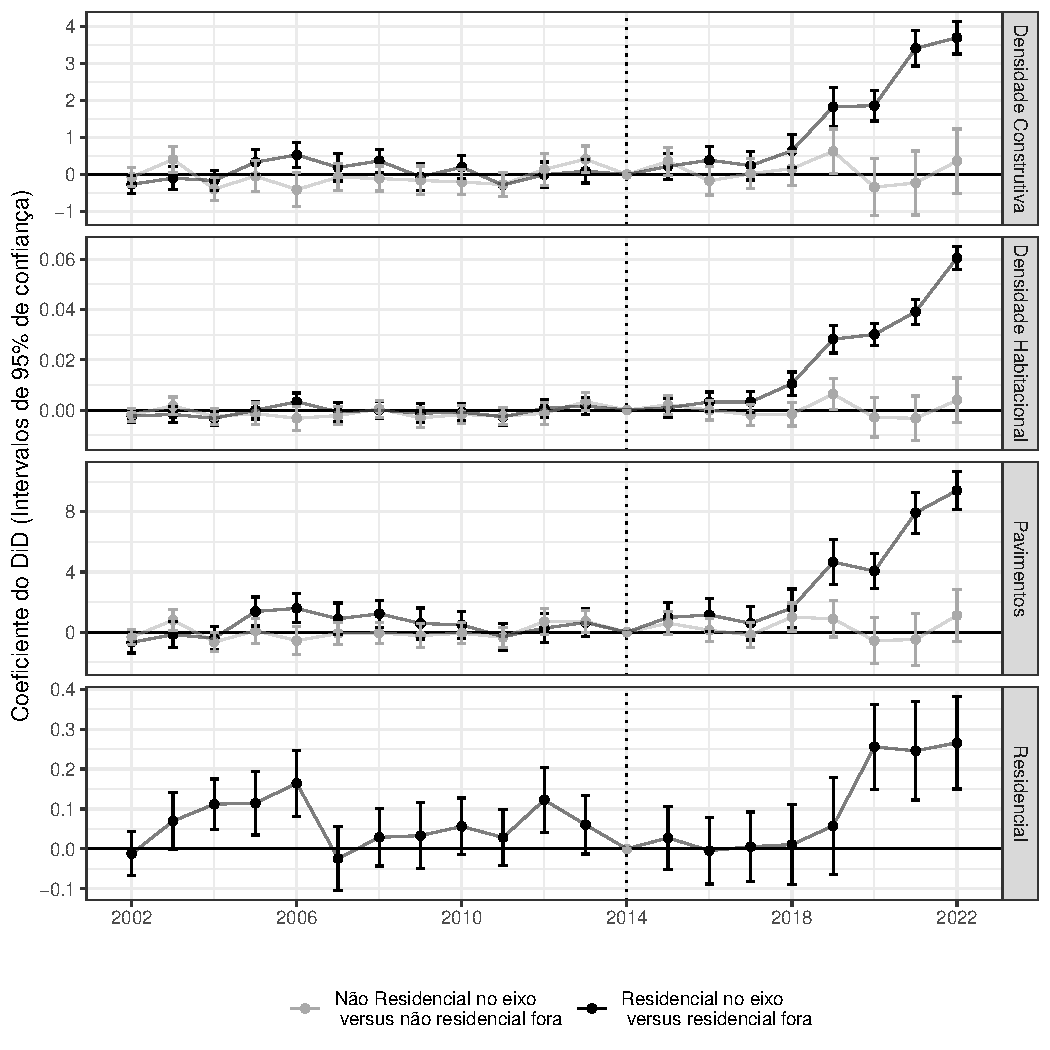
\includegraphics[width = .9\textwidth]{figuras/event-study.pdf}
    \label{fig:event-study}
\end{figure}

Para fortalecer a análise e identificar heterogeneidade temporal nos resultados, foi conduzido também um estudo de evento. Os resultados estão apresentados na Figura \ref{fig:event-study}. O \textit{Event study} também aponta para um aumento da densidade construtiva, densidade habitacional e pavimentos depois do PDE, mas o efeito parece se intensificar após 2018. Isso pode ser explicado pelo fato de que os empreendimentos entregues entre 2014 e 2017 em grande parte ainda seguiam a regulação do PDE de 2002. Além disso, foram observadas tendências paralelas no período pré PDE, indicando que de fato os grupos são comparáveis e o critério escolhido para separação dos grupos é exógeno. Por fim, um resultado surpreendente é de que os eixos parecem ter afetado apenas os empreendimentos residencias, tendo inclusive aumentado a probabilidade do tipo de uso construído no lote ser residencial.

\subsection{Abordagem de RDD}

Considerando o sucesso da metodologia de assumir como parecidos os grupos que estão próximos da fronteira dos eixos, a estratégia do RDD faz bastante sentido\footnote{Inclusive, o RDD se torna igual à estimação por diferença, quando o grau do polinômio é igual a zero e a \textit{bandwidth} é a mesma.}. A hipótese de identificação do RDD consiste em considerar que no entorno do ponto de corte, as observações imediatamente acima e abaixo do limiar são similares em todas as características observáveis e não observáveis, exceto pela variável de tratamento \cite{Cattaneo2019, Cattaneo2024}. Como discutido anteriormente, essa exogeneidade existe, visto que a diferença entre um lote de tratamento e o outro de controle é apenas atravessar a rua.

Entretanto, quando é implementado o RDD, não se observa efeito do tratamento -- este resultado pode ser visto na Figura \ref{fig:rdd-IPTU}. O motivo pelo qual isso acontece, é que como são poucos os lotes que receberam edificação pós PDE (consultar Figura \ref{fig:area-setor}), mesmo que este tenha um efeito significativo, ele é imperceptível quando se considera todos os lotes. O resultado torna-se significativo quando se seleciona apenas os lotes que receberam edificação após 2014. Neste caso, é observado um aumento na densidade construtiva, densidade habitacional e pavimentos (Figura \ref{fig:rdd-IPTU-posPDE}). 

\begin{figure}[!h]
    \centering

    \caption{RDD para os padrões construtivos no entorno dos eixos}
    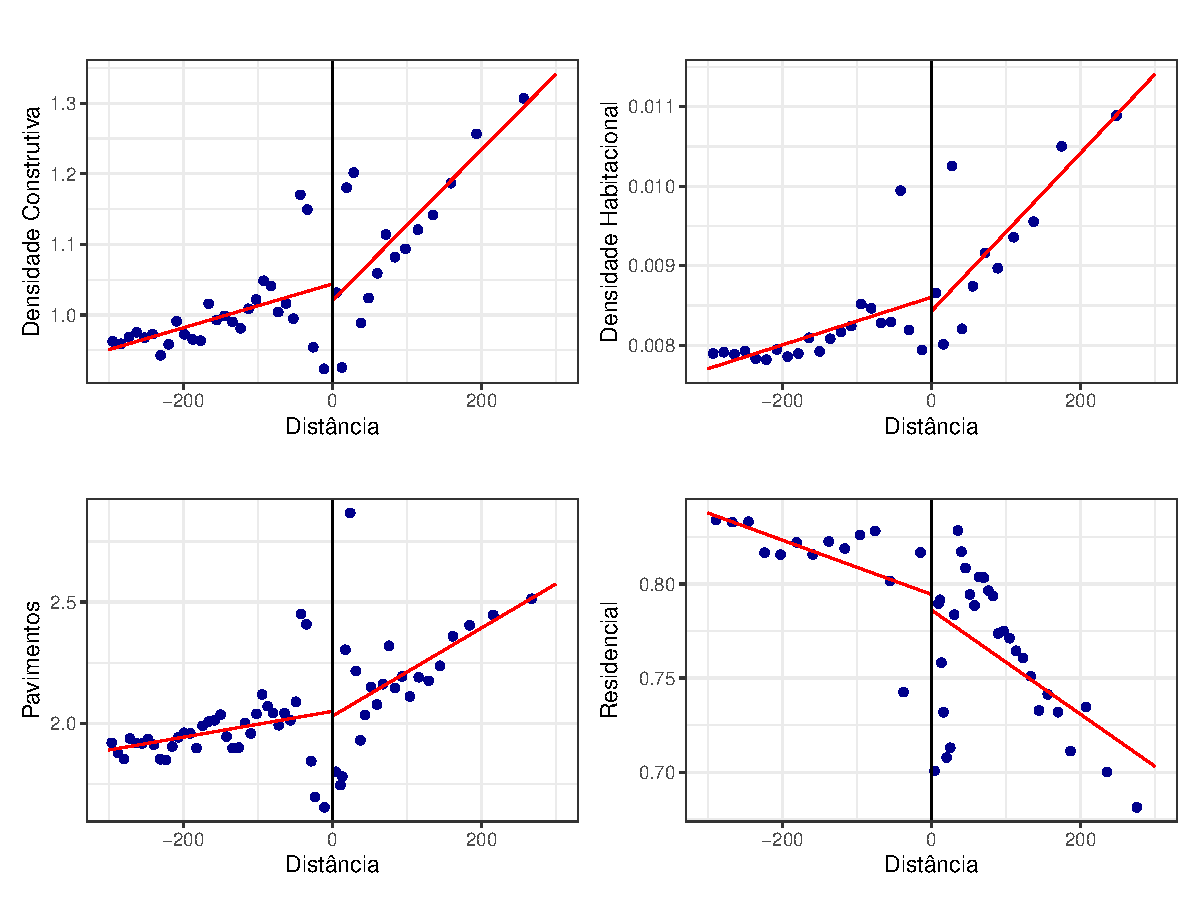
\includegraphics[width = .9\textwidth]{figuras/rdd-plot-IPTU.pdf}
    \label{fig:rdd-IPTU}

    \caption{RDD para os padrões construtivos no entorno dos eixos, filtrando por lotes com edificações recentes}
    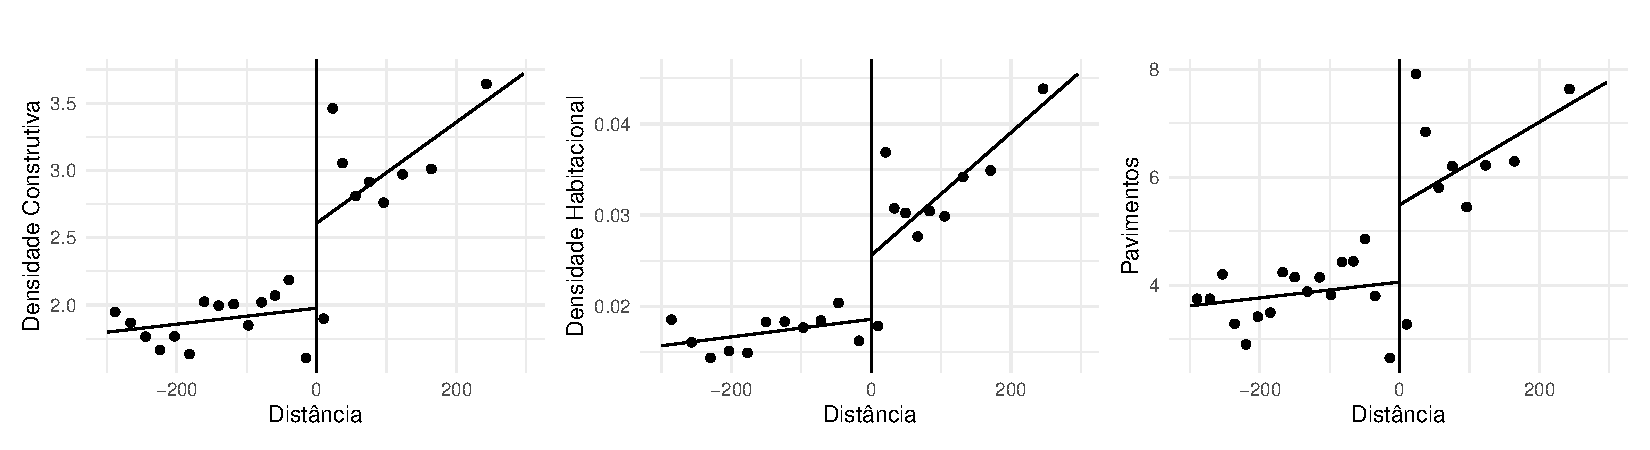
\includegraphics[width = .9\textwidth]{figuras/rdd-plot-IPTU-posPDE.pdf}
    \label{fig:rdd-IPTU-posPDE}
\end{figure}


Na Tabela \ref{tab:rdd-IPTU} é possível observar os resultados do RDD filtrado apenas para lotes com edificações novas e utilizando \textit{kernel} triangular com largura de banda escolhida automaticamente. Os resultados são semelhantes aos encontrados via diferenças em diferenças e os apresentados na Figura \ref{fig:rdd-IPTU-posPDE}, com exceção da probabilidade do lote ser residencial. Como teste placebo, foi replicado o mesmo procedimento, mas considerando o \textit{cutoff} em -100 ao invés de zero. A largura de banda selecionada automaticamente foi menor que 100, o que implica que nesse procedimento houve uma comparação do grupo controle com o próprio grupo controle. O teste placebo não apresentou efeito para os três componentes do padrão construtivo, validando o teste e trazendo mais evidências para a exogeneidade do tratamento na fronteira. Todavia, o coeficiente associado ao lote ser residencial apresentou significância, invalidando a inferência sobre esta variável da Tabela \ref{tab:rdd-IPTU}.

\begin{table}[h]
\centering
\caption{RDD results with only buildings from after the SMP (2014)} 
\fontsize{10pt}{12pt}\selectfont
\begin{tabular*}{.85\linewidth}{@{\extracolsep{\fill}}lccc}
\toprule
  & Densidade Construtiva & Densidade Habitacional & Pavimentos \\ 
\midrule\addlinespace[2.5pt]
Conventional & 0.707** & 0.010*** & 1.955** \\ 
Bias-Corrected & 0.638** & 0.010** & 1.821** \\ 
{Robust} & {0.638*} & {0.010*} & {1.821*} \\ 
\midrule
Observations (left)  & 622 & 799 & 624 \\ 
Observations (right) & 684 & 841 & 689 \\ 
Bandwidth & 61.2 & 76.3 & 61.7 \\ 
\bottomrule
\end{tabular*}
\begin{minipage}{.85\linewidth}
+ p < 0.1, * p < 0.05, ** p < 0.01, *** p < 0.001\\
\end{minipage}
\label{tab:rdd-IPTU}
\end{table}



\begin{table}[h]
  \centering
\caption{RDD placebo test with the cutoff 100 meters outside the axis region} 
\fontsize{10pt}{12pt}\selectfont
\begin{tabular*}{.85\linewidth}{@{\extracolsep{\fill}}lccc}
\toprule
  & Building Density & Dwelling Unit Density & Storeys \\ 
\midrule\addlinespace[2.5pt]
Conventional & 0.031 & 0.000 & 0.211 \\ 
Bias-Corrected & 0.096 & 0.001 & 0.407 \\ 
{Robust} & {0.096} & {0.001} & {0.407} \\ 
\midrule
Observations (left) & 863 & 921 & 890 \\ 
Observations (right) & 990 & 1070 & 1027 \\ 
Bandwidth & 76.9 & 82.7 & 79 \\ 
\bottomrule
\end{tabular*}
\begin{minipage}{.85\linewidth}
+ p < 0.1, * p < 0.05, ** p < 0.01, *** p < 0.001\\
\end{minipage}
\end{table}




\subsection{Resultados principais}

Os dados mostram que construções nos eixos após o início da vigência do PDE apresentam maior densidade construtiva, densidade habitacional e pavimentos. As evidências apontam também para uma intensificação do efeito do PDE começando a partir de 2018 e alcançando seu ápice nos dados mais recentes, em 2022. Além disso, as mudanças do PDE parecem ter afetado apenas os empreendimentos residenciais, enquanto nos outros usos não se observa uma diferença significativa entre a região de eixo e fora dos eixos.

Entretanto, um resultado que se destaca também é que a mudança causada pelo PDE nos últimos 10 anos não apresentou intensidade e/ou velocidade suficientes para se observar uma divisão territorial clara de eixo e não eixo nos padrões construtivos. Para observar os resultados, é necessário olhar exclusivamente para os novos empreendimentos, que, como representado na Figura \ref{fig:area-setor}, representam menos de 5\% dos empreendimentos.

\clearpage
\section{Da regulação à densidade populacional}
\label{sec:perg3}

O objetivo desta seção é responder: \textbf{A regulação foi capaz de influenciar a densidade populacional na cidade?} Como comentado na Seção \ref{sec:perg1}, a densidade habitacional é o componente mais importante para determinar a densidade populacional, e segundo os resultados apresentados na Seção \ref{sec:perg2} os eixos causaram um aumento da densidade habitacional. Dessa forma, a hipótese que mais faz sentido é que a densidade populacional nos eixos aumentou. Para testar esta hipótese foi realizado um procedimento parecido com o apresentado na Seção \ref{sec:perg2}, mas trocando a variável resposta por densidade populacional.

A principal diferença é que, no caso da densidade, a unidade de observação (setor censitário) é geograficamente muito maior do que os lotes. Assim, é comum que um setor censitário próximo à fronteira ocupe tanto áreas do grupo de controle quanto do grupo de tratamento, o que exige sua exclusão da análise. No entanto, a ocorrência desse fenômeno é tão frequente que, nas proximidades imediatas da fronteira, há um número insuficiente de unidades para realizar a análise usando RDD. Esse fenômeno é ilustrado na Figura \ref{fig:rdd-densidade-censo}. 

Além disso, há um viés de sobrevivência, no qual apenas setores censitários pequenos, com menor probabilidade de estarem em ambos os lados da fronteira, permanecem próximos à borda após aplicar o critério de exclusão\footnote{No caso do setor censitário, é considerado de tratamento quando seu centroide está na região de eixo e mais de 95\% de sua área está nessa região. O controle é definido pela presença do centroide fora do eixo e menos de 5\% de área de eixo. Qualquer setor censitário que não cumpre com algum dos critérios é excluído}. O problema com esses setores é que, como discutido na Seção \ref{sec:dadosCenso}, quanto menor o setor censitário, maior tende a ser sua densidade, o que faz com que a densidade média na fronteira aumente de forma atípica tanto no grupo de controle quanto no de tratamento. Esses fatores inviabilizam a análise via RDD.

\begin{figure}[!h]
    \centering
    \caption{Número de observações por grupo em função da distância à fronteira do eixo}
    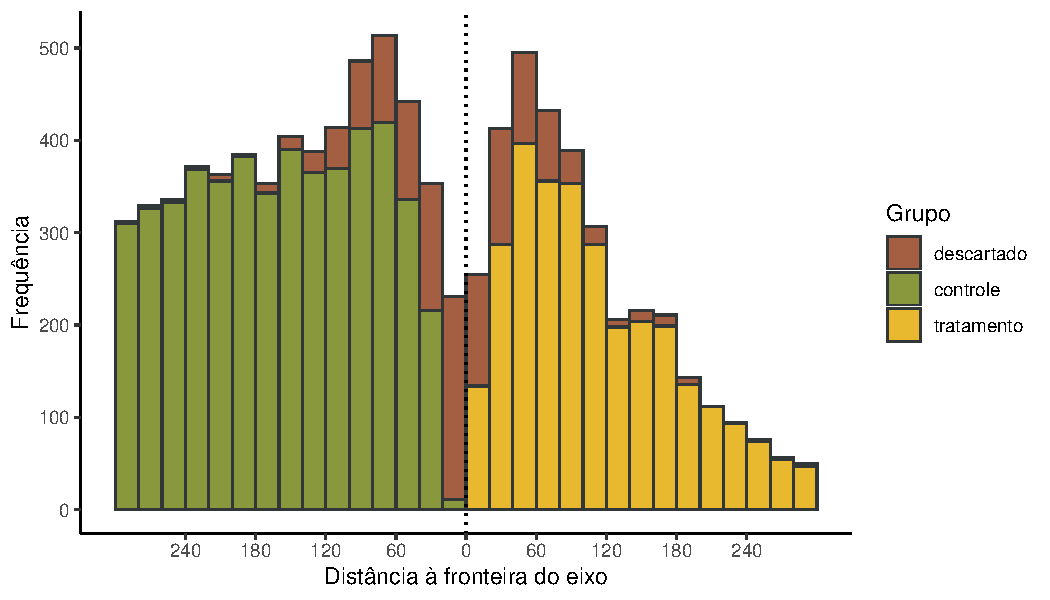
\includegraphics[width = .75\textwidth]{figuras/rdd-balanceamento-censo.pdf}
    \label{fig:rdd-densidade-censo}
\end{figure}

Como feito na Seção \ref{sec:perg2}, é possível obter alguns resultados preliminares antes de construir os modelos de regressão. Ao observar o número de habitantes na fronteira do eixo (50m de distância), é possível perceber, como apresentado na Tabela \ref{tab:censo-descritivo}, que as regiões de tratamento apresentaram um aumento populacional superior entre 2010 e 2022. Apesar de não conferir inferência causal, este resultado apoia a hipótese do adensamento em decorrência da regulação nos eixos.

\begin{table}[h]
    \centering
    \caption{Population before and after the SMP in each part of the city}
    {\small
    \begin{tabular}{
        >{\raggedright\arraybackslash}p{0.15\linewidth} 
        >{\raggedleft\arraybackslash}p{0.15\linewidth} 
        >{\raggedleft\arraybackslash}p{0.15\linewidth} 
        >{\raggedleft\arraybackslash}p{0.15\linewidth}}
        % \toprule
        \textbf{Region} & \textbf{2010} & \textbf{2022} & \textbf{$\Delta$} \\
        \midrule
        Outside axis & 9.795.114 & 10.192.905 & +397.791 \\
        Inside axis & 1.414.559 & 1.259.094 & -155.465 \\
    \end{tabular}
    }
    \label{tab:censo-descritivo}
\end{table}

\subsection{Abordagem via diferenças em diferenças}

A estratégia de identificação se mantém a mesma da Seção \ref{sec:perg2}, na qual foram considerados apenas os setores censitários na proximidade da fronteira do eixo, onde a diferença entre o controle e o tratamento é apenas atravessar a rua. A partir disso, foi conduzido um \textit{diff-in-diff} com efeito fixo de ano e também com efeito fixo de setor censitário. Os resultados podem ser observados na Tabela \ref{tab:did-censo}. As regressões das colunas (A) e (C) apresentam dados do tipo \textit{pooled} com efeito fixo apenas de ano e grupo, enquanto nas colunas (B) e (D) são em painel e efeito fixo tanto de ano quanto de setor censitário. Aproximadamente 90\% dos setores censitários analisados na região mudam de posição e/ou tamanho entre 2010 e 2022, mas os 10\% que mantém a mesma forma podem ser comparados no tempo\footnote{Enquanto o Censo de 2010 apresentava 18.953 setores censitário, o de 2022 conta com 27.592, o que implica que a malha se alterou significativamente}, possibilitando a análise em painel. 

\begin{table}[!t]
\caption{Resultado diff-in-diff do Censo, para setores censitários em um raio de 100m dos eixos} 
\centering
\fontsize{12.0pt}{14.4pt}\selectfont
\begin{tabular*}{.7\linewidth}{@{\extracolsep{\fill}}lcc}
  & (A) & (B) \\ 
\midrule\addlinespace[2.5pt]
Intercepto & 0.057*** & 0.050*** \\ 
T (Grupo de tratamento) & -0.003 & 0.000 \\ 
P (Período pós PDE) & -0.015*** & -0.011** \\ 
Q (Percentual residencial novo) &  & 0.108*** \\ 
T x P & -0.001 & -0.004 \\ 
T x Q &  & -0.055* \\ 
P x Q &  & -0.045* \\ 
{T x P x Q} & {} & {0.043} \\ 
\midrule
Num.Obs. & 3217 & 3217 \\ 
R2 & 0.013 & 0.040 \\ 
R2 Adj. & 0.012 & 0.037 \\ 
\bottomrule
\label{tab:did-censo}
\end{tabular*}
\begin{minipage}{.7\linewidth}
+ p < 0.1, * p < 0.05, ** p < 0.01, *** p < 0.001\\
\end{minipage}
\end{table}



As evidências demonstradas na Tabela \ref{tab:did-censo} apontam para o aumento da densidade populacional por decorrência da regulamentação dos eixos, apesar da signifância apenas de 5\%. Em termos práticos, as estimativas para o aumento populacional são de aproximadamente 5.000 habitantes por quilômetro quadrado em relação ao grupo controle (Coluna B). Como referência, a média de moradores dos setores censitários considerados no raio de 50m da fronteira dos eixos em 2022 foi de 48.397 habitantes. Entretanto, é importante notar que este efeito foi estimado de maneira local e não pode ser extrapolado para o restante da cidade. Os resultados são robustos para diferentes recortes de distância, caso seja incorporado o efeito fixo de setor censitário. Os coeficientes da regressão podem ser analisados na Figura \ref{} do Apêndice \ref{} para diferentes recortes de distância.

\subsection{Resultados principais}

Os resultados da análise indicam que a densidade populacional nos eixos de transporte aumentou após a implementação das regulamentações, conforme previsto nas hipóteses iniciais. Este resultado está em conformidade com as conclusões trazidas nas Seções \ref{sec:perg1} e \ref{sec:perg2}, que permitiram compreender que o principal componente do adensamento populacional, que é a densidade habitacional, apresentou um aumento significativo na região dos eixos.

\chapter{Conclusão}
\label{chp:conclusao}

\section{Resultados principais}
\label{sec:conclusao}

A partir dos resultados obtidos, foi possível decompor a análise em três aspectos fundamentais, conforme estruturado na Figura \ref{fig:diagrama}: (i) a relação entre os instrumentos regulatórios e os padrões construtivos, (ii) a eficácia desses padrões em gerar a densidade populacional esperada e (iii) a relação final entre regulação e densidade populacional.

Em primeiro lugar, os instrumentos regulatórios introduzidos pelo plano diretor de 2014, mostraram-se eficazes em modificar os padrões construtivos nos EETUs. A análise por diferenças em diferenças (DiD) revelou que, após a implementação do PDE, principalmente a partir de 2018, os eixos de transporte atraíram empreendimentos com maior densidade construtiva, densidade habitacional e pavimentos por edificação. A regressão em descontinuidade (RDD) complementa esses achados com estimativas parecidas. Esses resultados sugerem que a regulação urbana nos eixos atuou conforme esperado em termos de mudança de padrão construtivo. No entanto, a velocidade em que essa mudança ocorre ainda não foi suficiente para observar uma descontinuidade espacial na fronteira dos eixos\footnote{Se a informação sobre o ano em que o lote foi edificado fosse ocultada, não seria possível descobrir, apenas observando os padrões construtivos, onde se encontra a fronteira do eixo na maior parte da cidade}.

Em segundo lugar, ao avaliar a capacidade desses padrões construtivos de gerar a densidade populacional esperada, os resultados destacaram a densidade habitacional como o principal determinante da densidade populacional. A análise evidencia que a cota parte - responsável por definir um número mínimo de unidades habitacionais - tem uma influência mais direta sobre o aumento de moradores nas áreas de eixo do que os instrumentos de CA e gabarito. Em contraste, a verticalização apresentou uma relação negativa com a densidade populacional quando são mantidas constantes a densidade construtiva e habitacional, evidenciando a associação entre empreendimentos verticais e núcleos familiares menores. 

Por fim, ao ligar os pontos e observar o impacto da regulação sobre a densidade populacional nos EETUs, as evidências sugerem que a política implementada pelo PDE de fato resultou em um aumento na ocupação populacional dessas áreas. Portanto, o PDE, por meio dos instrumentos de regulação conseguiu direcionar o adensamento populacional, ainda que com intensidade moderada, para as zonas no entorno do transporte público de alta capacidade, que era seu objetivo principal.  

\section{Contribuições para o debate público}
\label{sec:contribuicoes}

Ainda que o PDE tenha alcançado seu objetivo de adensar as áreas de eixos, é essencial destacar os pontos fortes e as limitações dos mecanismos utilizados. A previsão da vigência do PDE é até 2029, então trazer evidências para o debate público é de suma importância para que as decisões que forem feitas para o PDE de 2030 sejam baseadas em fatos.

Dentre os acertos, com base nos resultados apresentados, a introdução da cota parte foi determinante para o sucesso do adensamento nos eixos, despertando interesse em entender como otimizar o uso desse instrumento. No PDE de 2014, apenas as regiões de eixos tiveram a cota parte regulamentada, enquanto o restante da cidade ficou sem limites máximos -- uma decisão que poderia ser reconsiderada, dada a eficácia do instrumento. Além disso, é importante investigar se o valor de 20 é realmente ideal para a cota parte nas áreas de eixos. 

Considerando o objetivo de adensar a região dos eixos, remover os limites de gabarito foi um erro. As evidências apontam que para um dado CA e cota parte, quanto maior for a verticalização, menos pessoas vão habitar o empreendimento em média. Isso acontece, pois quando se fixa o número de unidades habitacionais e os metros quadrados construídos, há uma relação inversa entre a verticalização e a taxa de ocupação: quanto mais vertical, menos área é ocupada e maiores são os recuos. Nesse sentido, teria sido mais adequado permitir um CA ilimitado, enquanto o gabarito mantém-se mais restritivo.

Por fim é importante destacar que o efeito do PDE não foi incentivar o adensamento, mas sim, permitir que ele ocorra. O CA permitido nos eixos, por exemplo, passou a ser entre 2 a 4, mas dentro desse intervalo não há incentivos para que se chegue mais perto de 4. Inclusive, há um desincentivo ao adensamento construtivo, visto que na medida em que se constrói a mais do que o CA básico, os impostos aumentam. Um fenômeno parecido incorre sobre a cota parte, que apresenta um máximo de 20 ao invés de incentivos para que seja pequena. A peculiaridade desse sistema de limitações ao invés de incentivos advém da resposta do mercado imobiliário às regras do jogo. Como as mudanças na regulação não permitem um lucro maior e, em algumas casos causa uma redução dele, a oferta de habitação diminui, o que caminha na direção oposta aos objetivos do PDE.
